% IEEE conference template
\documentclass[conference]{IEEEtran}
\usepackage{cite}
\usepackage{amsmath,amssymb,amsfonts}
\usepackage{algorithmic}
\usepackage{graphicx}
\usepackage{textcomp}
\usepackage{xcolor}
\def\BibTeX{{\rm B\kern-.05em{\sc i\kern-.025em b}\kern-.08em
    T\kern-.1667em\lower.7ex\hbox{E}\kern-.125emX}}
\begin{document}

\title{AE 598 RL: DQN}

\author{
\IEEEauthorblockN{Rahil Makadia}
\IEEEauthorblockA{\textit{Department of Aerospace Engineering} \\
\textit{University of Illinois at Urbana-Champaign}\\
Urbana, IL, USA \\
makadia2@illinois.edu}
}

\maketitle

\section{Introduction}
This assignment focused on implementing a Deep Q-Network (DQN) algorithm on an environment consisting of a inverse pendulum problem. Different versions of the DQN algorithm were implemented and compared to each other. More specifically, the choice between algorithms was whether how often to update a target Q network or how to implement experience replay. Results show that the experience replay flag has the more significant influence and that experience replay gives better results in the inverse pendulum problem.

\section{Methods}
The Deep Q-Network used in this work is based on the work of Minh et al. (2015)\cite{b1}. The value function approximated by the deep neural network can be written as:
\begin{equation}
    Q^*=\max _\pi \mathbb{E}\left[r_t+\gamma r_{t+1}+\gamma^2 r_{t+2}+\ldots \mid s_t=s, a_t=a, \pi\right]
\end{equation}
where $Q$ is the value function, $s$ is the state, $a$ is the action, $r$ is the reward, $\gamma$ is the discount factor, and $\pi$ is the policy.

Two neural networks are used in the DQN algorithm. The first neural network is the Q network which is used to approximate the value function. The second neural network is the target Q network which is used to calculate the target value function. The neural networks used in this work had two hidden layers with 64 units each activated using a hyperbolic tangent function. The loss function for the neiral network is Mean Squared Error (MSE) and the RMSProp optimizer was used with a learning rate of 0.00025.

Another aspect of the DQN algorithm is the experience replay. This involves sampling minibatches of "experience" from a replay memory. One experience tuple consists of a state, action, reward, and next state. A minibatch is sampled from the replay memory every time the Q network needs to be updated. The target value function is calculated using the target Q network. In the standard DQN algorithm shown here, the target Q network is updated every 1000 steps. Table 1 shows the hyperparameters used in this work.

\begin{table}[htbp]
\centering
\caption{Hyperparameters}
\begin{tabular}{|c|c|}
\hline
\textbf{Hyperparameter} & \textbf{Value} \\ \hline
Number of episodes & 150 \\ \hline
Number of steps per episode & 100 \\ \hline
Learning rate & 0.00025 \\ \hline
$\gamma$ & 0.95 \\ \hline
Starting $\epsilon$ & 1.0 \\ \hline
Ending $\epsilon$ & 0.1 \\ \hline
Batch size & 32 \\ \hline
Replay memory size & 100000 \\ \hline
Target network update frequency & 1000 \\ \hline
\end{tabular}
\end{table}

However, there are cases where the target network is updated every step. In this case the DQN algorithm is essentially operating without a target network since its weights are the same as the main Q network. Another variation of the standard DQN algorithm used in this work was to not have experience replay, i.e., instead of smapling from a memory buffer, the minibatch is sampled from the current state, action, reward, and next state.

\section{Results}
\subsection{DQN Algorithm}
The standard DQN algorithm was run first for 150 episodes to ensure correctness of the algorithm. The results are shown in Fig. \ref{fig:yes_target_yes_replay_one_run}.

\begin{figure}[h]
\centering
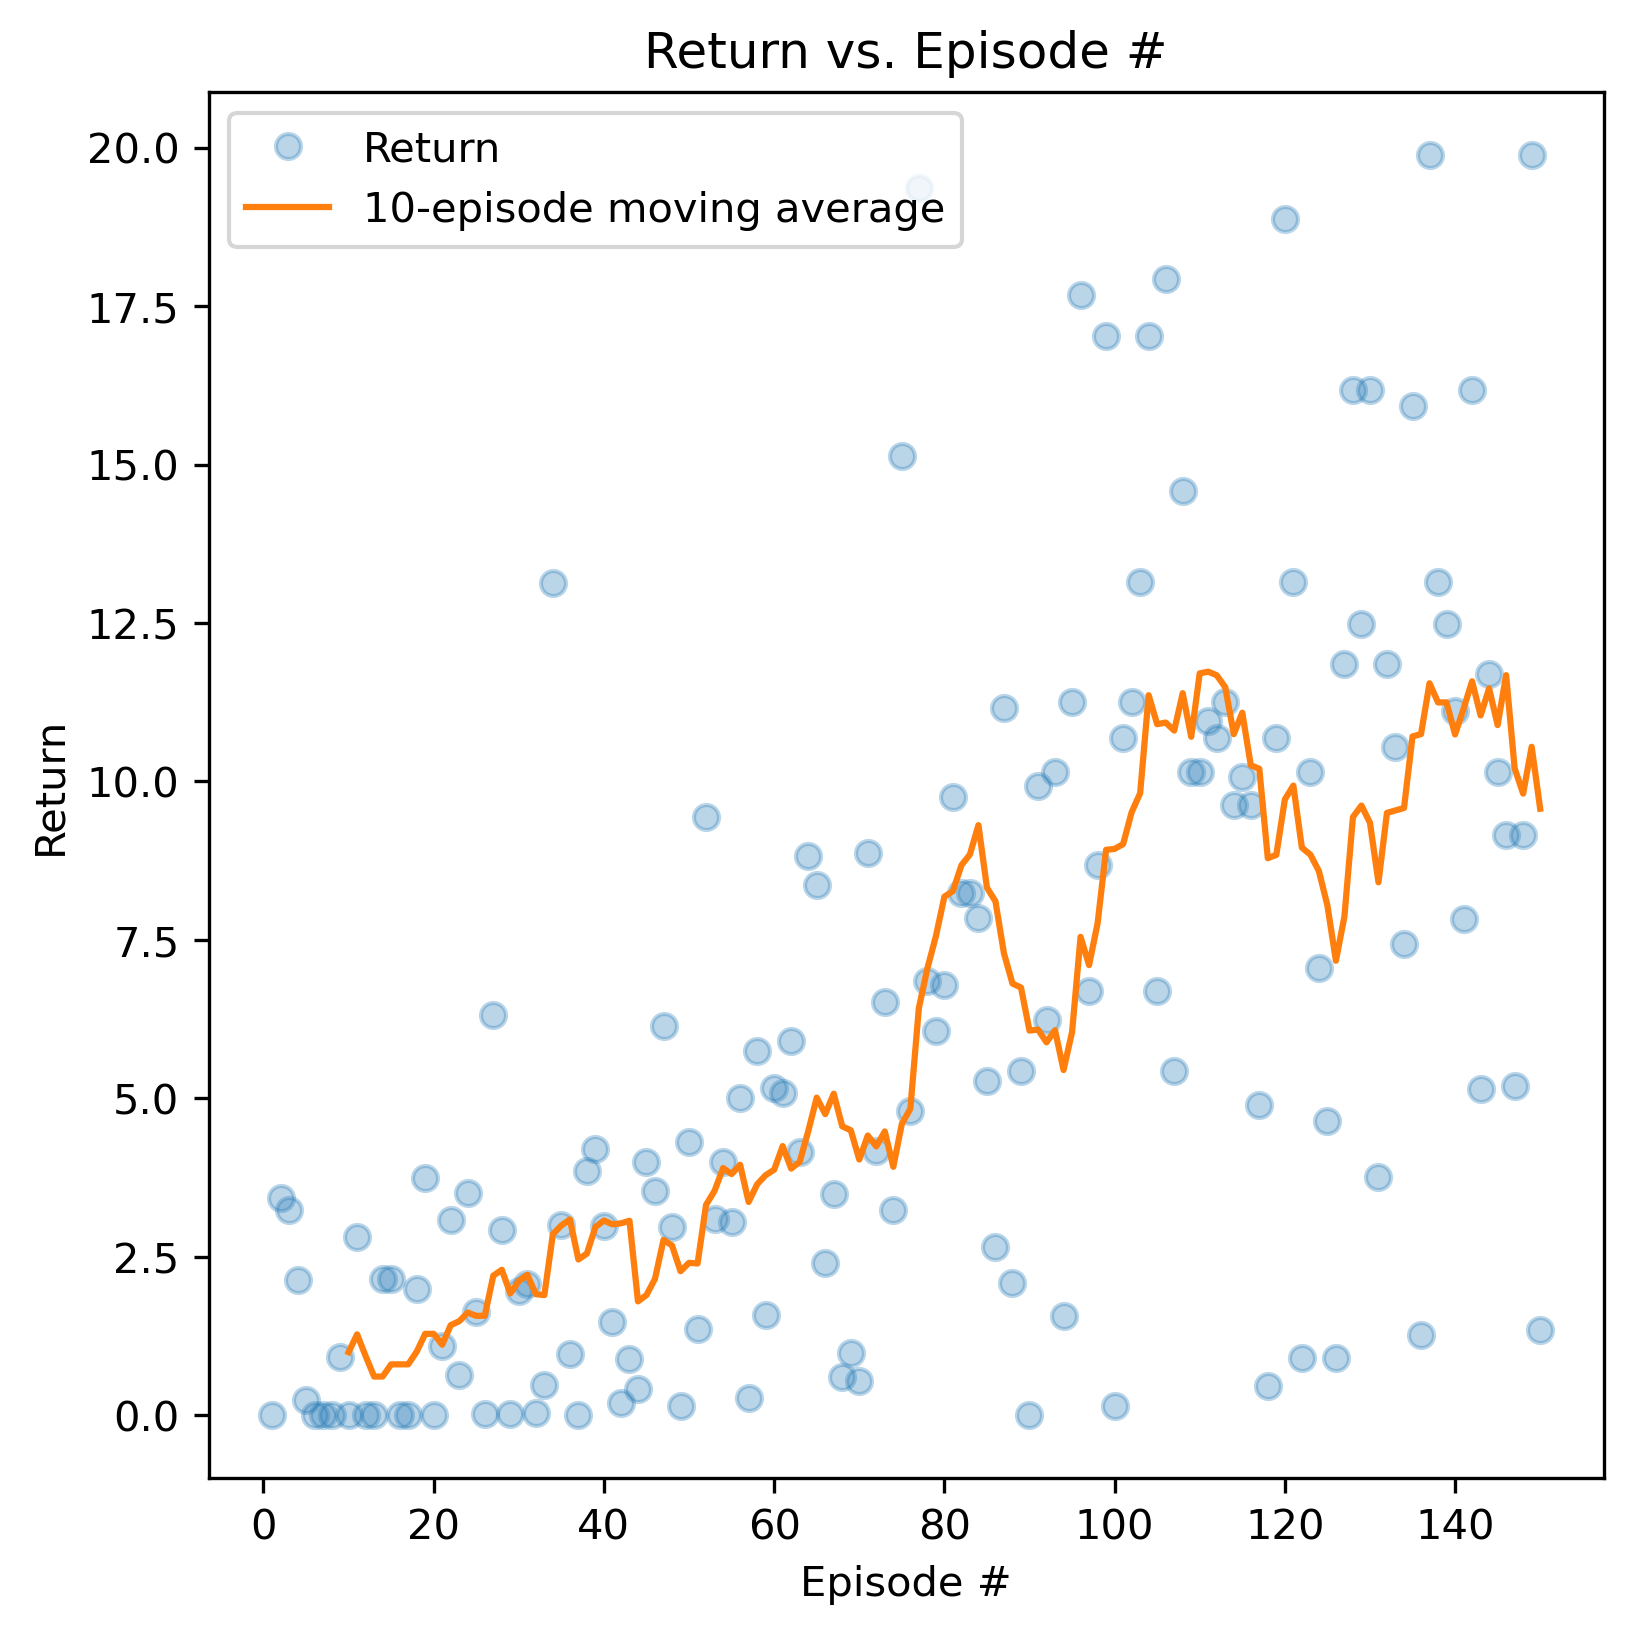
\includegraphics[width=\linewidth]{../figures/yes_target_yes_replay/return_150_1000.png}
\caption{Learning curve for one run of the standard DQN algorithm}
\label{fig:yes_target_yes_replay_one_run}
\end{figure}
To ensure that this onse run was not an outlier, the standard DQN algorithm was run 10 times and the mean return and 1-sigma bounds are shown in Fig. \ref{fig:yes_target_yes_replay_10_runs}.

\begin{figure}[h]
\centering
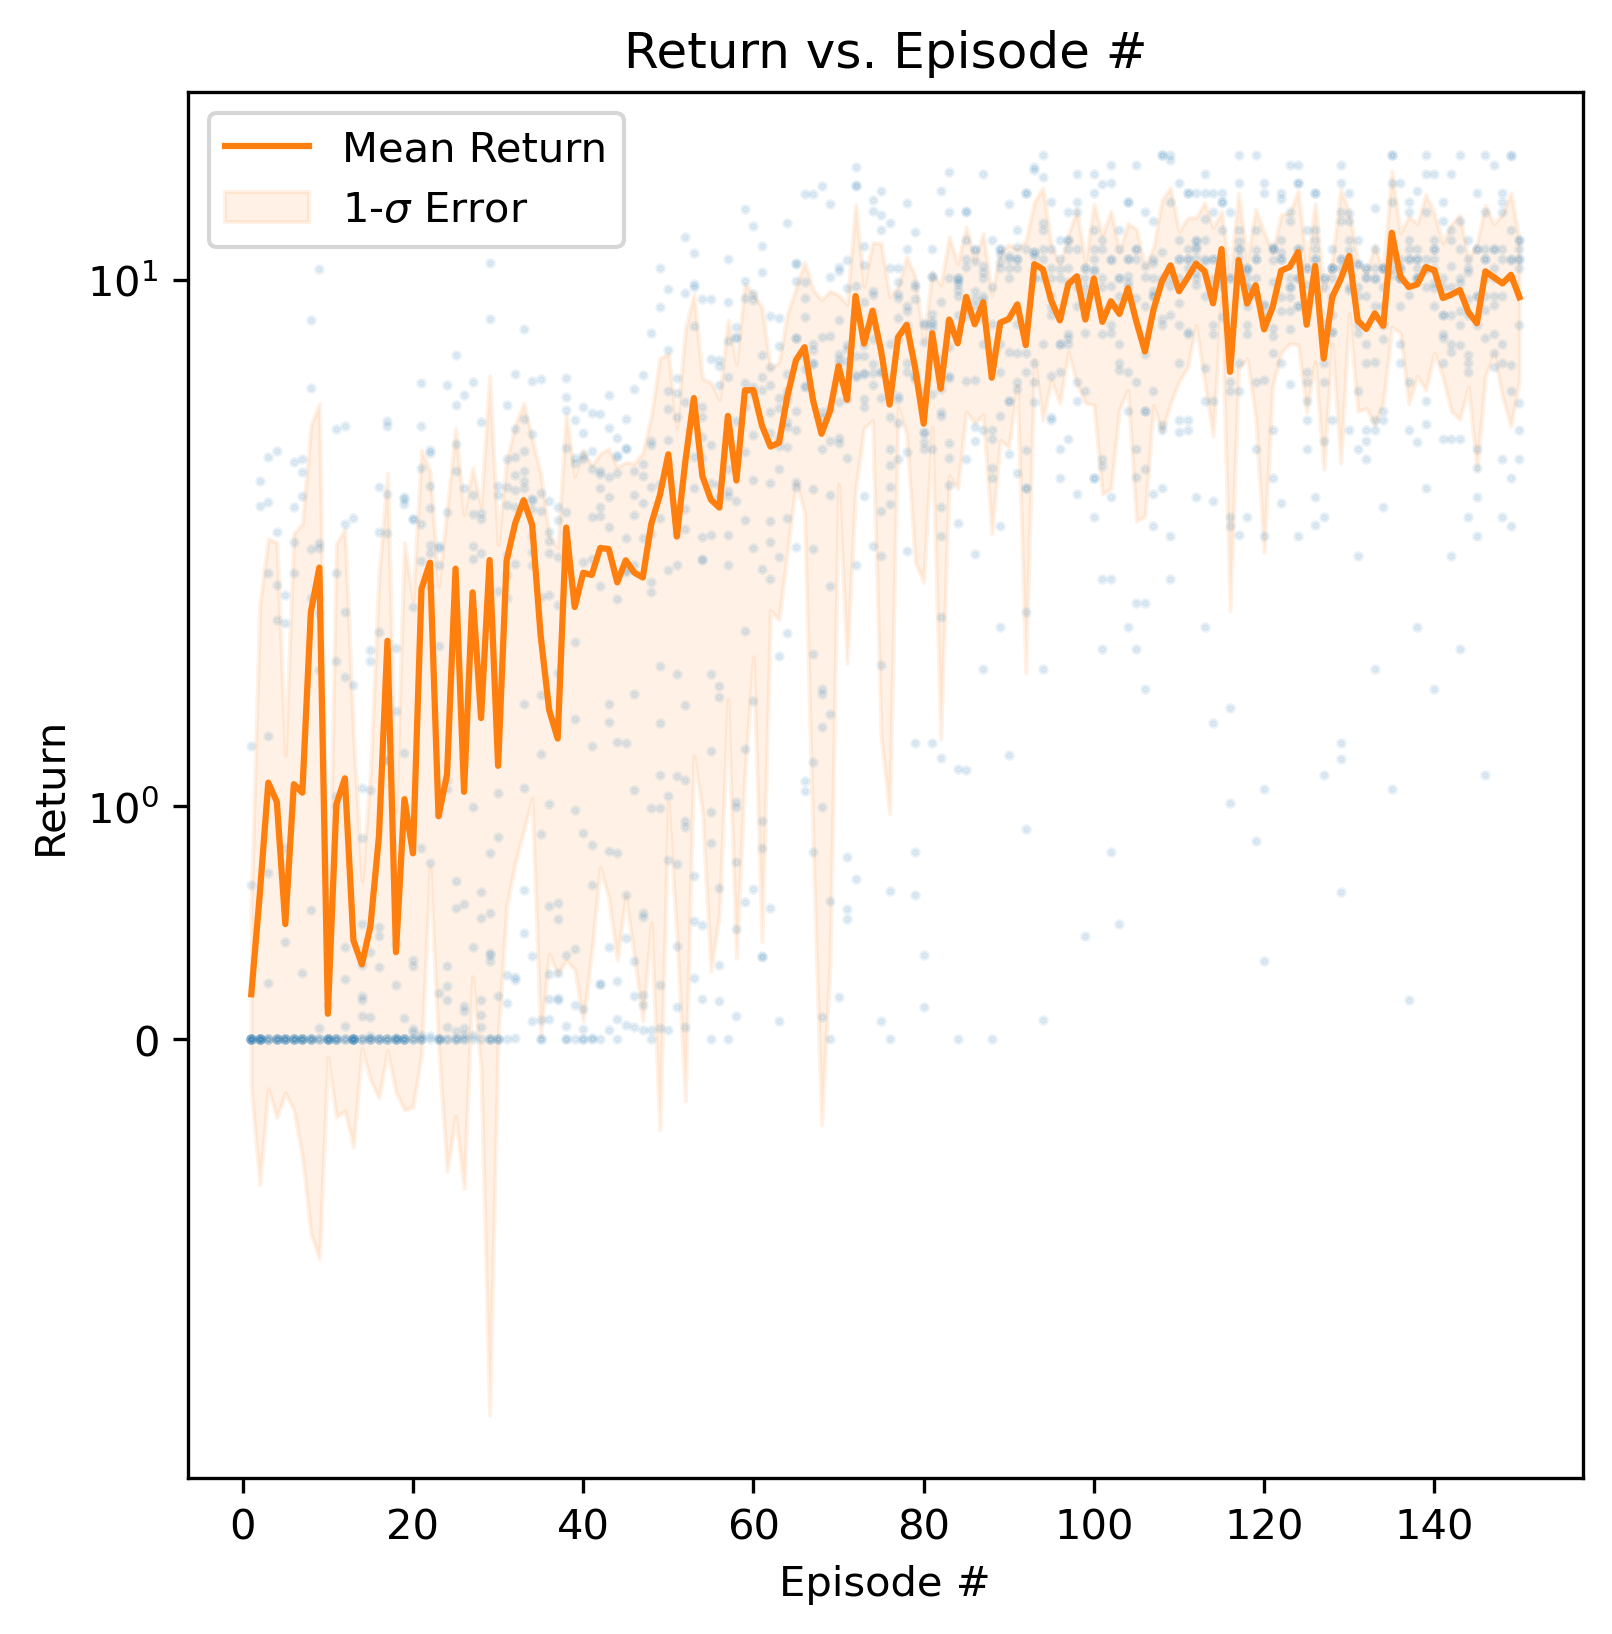
\includegraphics[width=\linewidth]{../figures/yes_target_yes_replay/mean_return_150_1000_log_True.png}
\caption{Mean return and 1-sigma bounds for 10 runs of the standard DQN algorithm}
\label{fig:yes_target_yes_replay_10_runs}
\end{figure}
We see that the mean return for the 10-run case is around 10, which is the same as the single run case, and that the standard deviation shrinks towards the end of the learning curve. This is an indication that the network is learning the policy to keep the pendulum upright. This optimal policy is shown in Fig. \ref{fig:yes_target_yes_replay_policy}.

\begin{figure}[h]
\centering
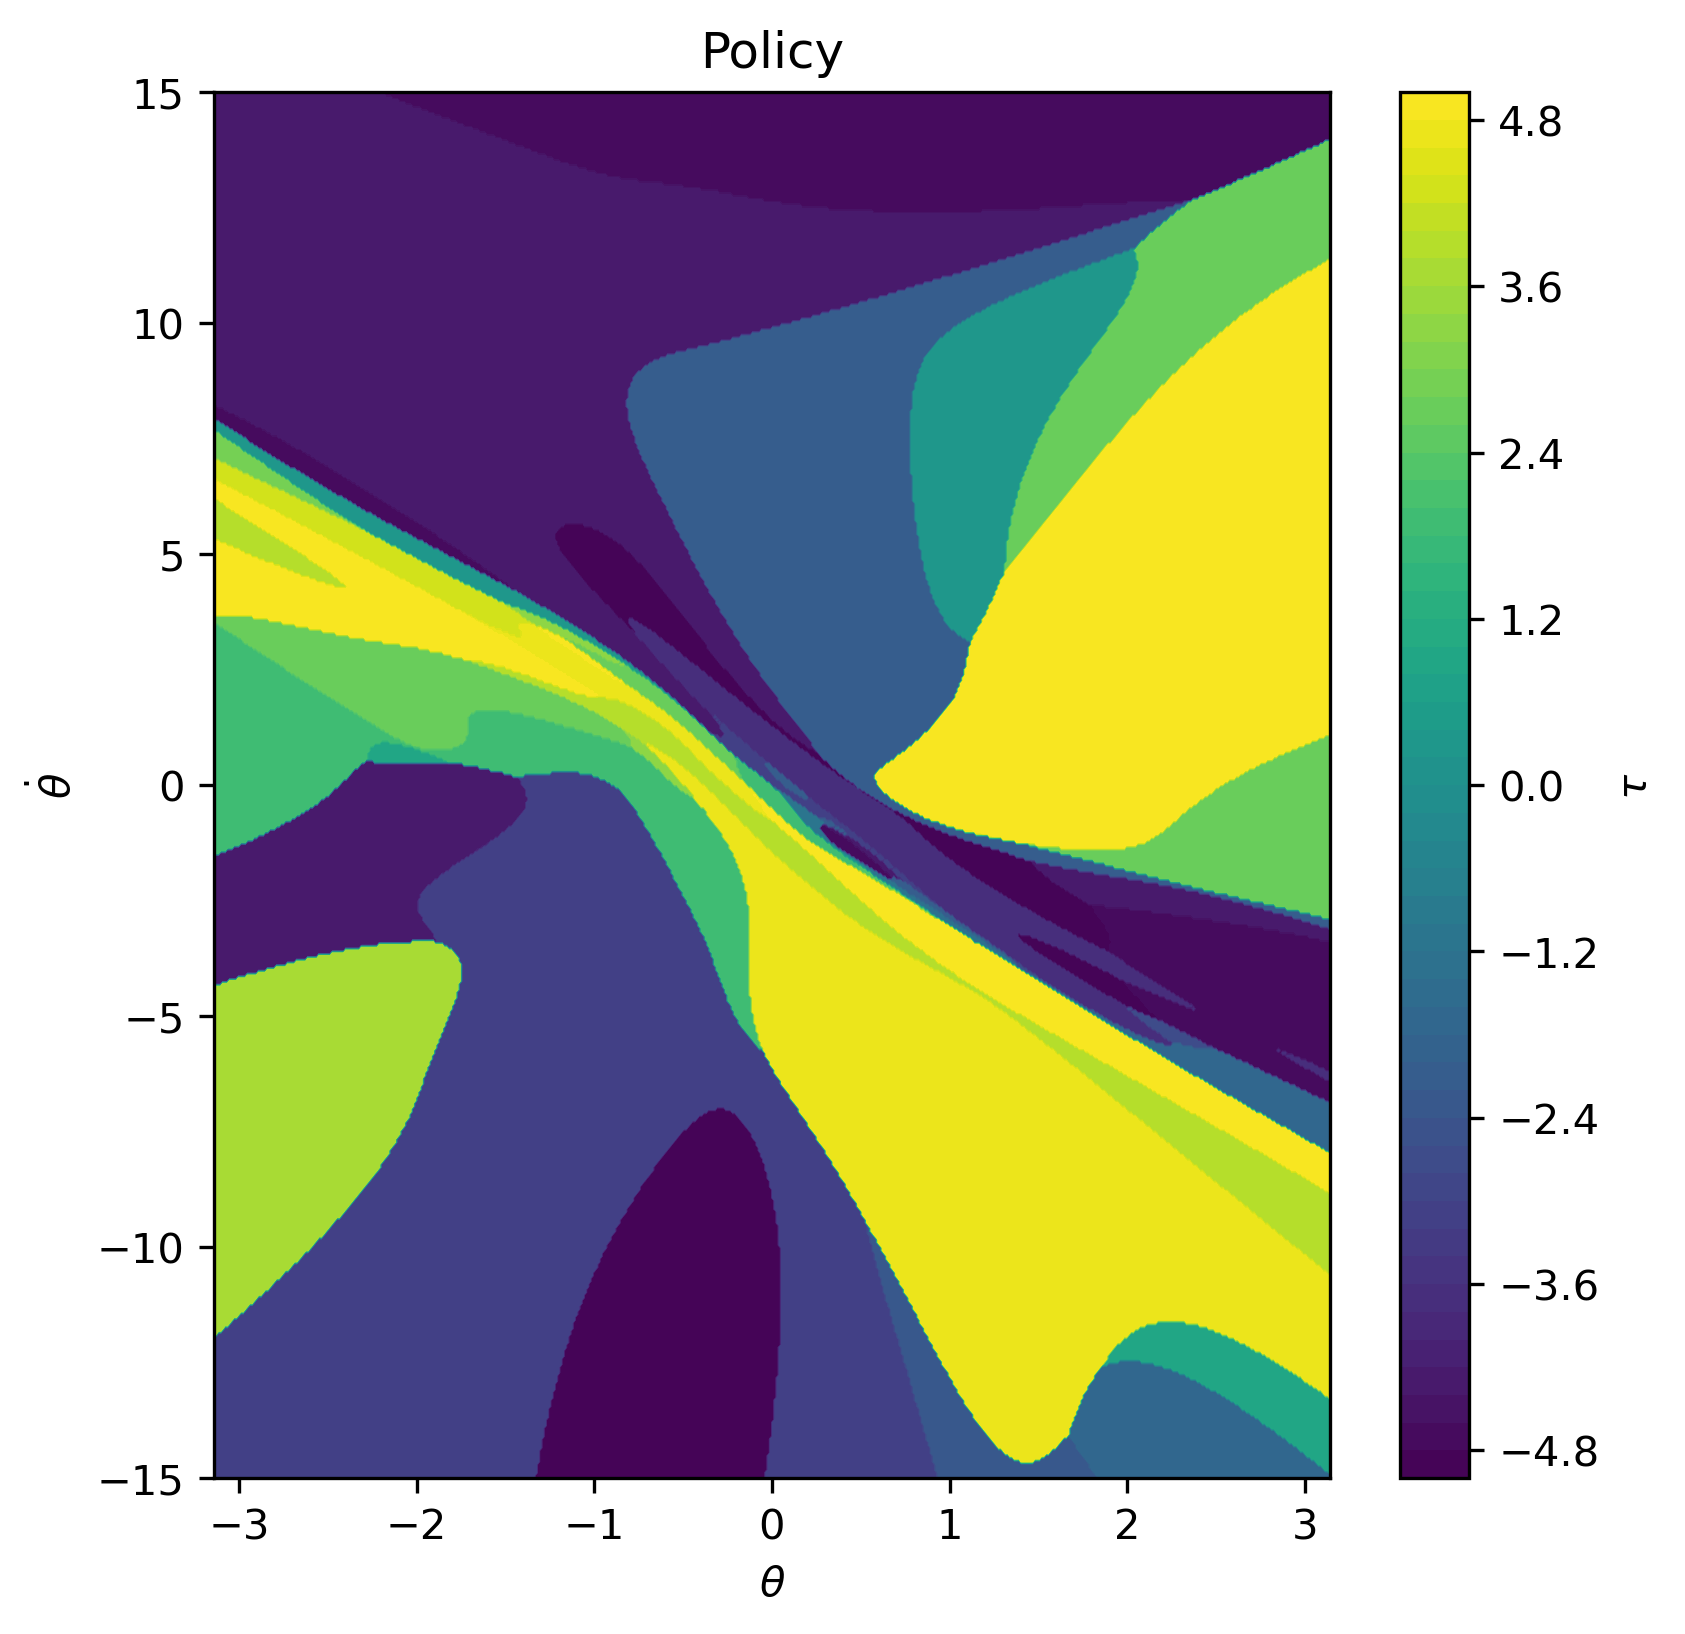
\includegraphics[width=0.949\linewidth]{../figures/yes_target_yes_replay/ctr_policy_150_1000.png}
\caption{Learned policy for the standard DQN algorithm}
\label{fig:yes_target_yes_replay_policy}
\end{figure}
Additionally, the value function and state evolution for one example episode are shown in Fig. \ref{fig:yes_target_yes_replay_value_function} and Fig. \ref{fig:yes_target_yes_replay_state_evolution}, respectively.

\begin{figure}[h]
\centering
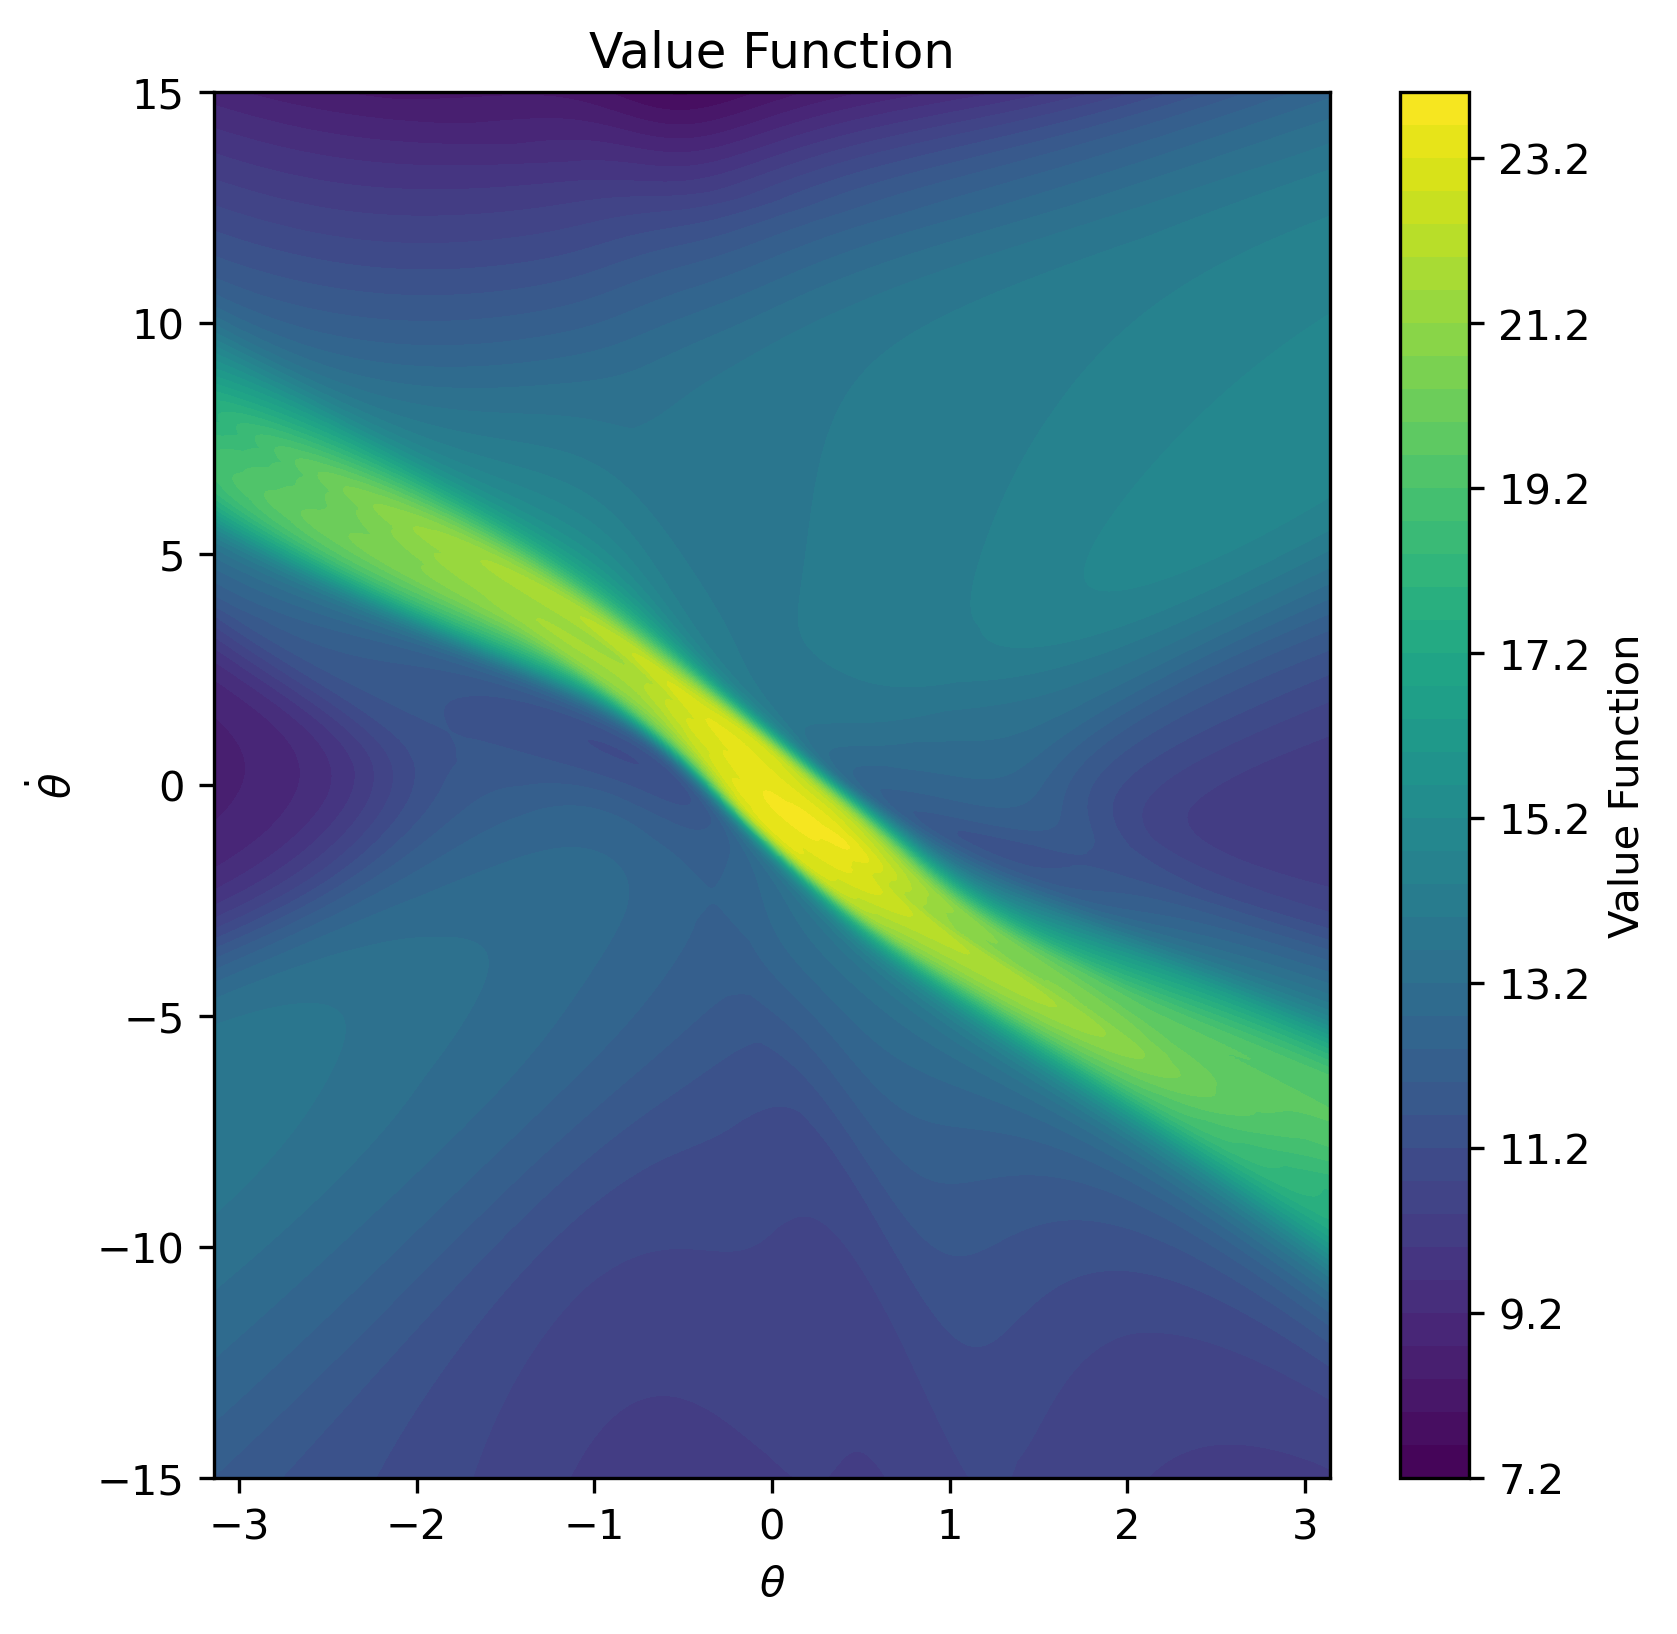
\includegraphics[width=\linewidth]{../figures/yes_target_yes_replay/ctr_value_func_150_1000.png}
\caption{Value function for the standard DQN algorithm}
\label{fig:yes_target_yes_replay_value_function}
\end{figure}
\begin{figure}[h]
\centering
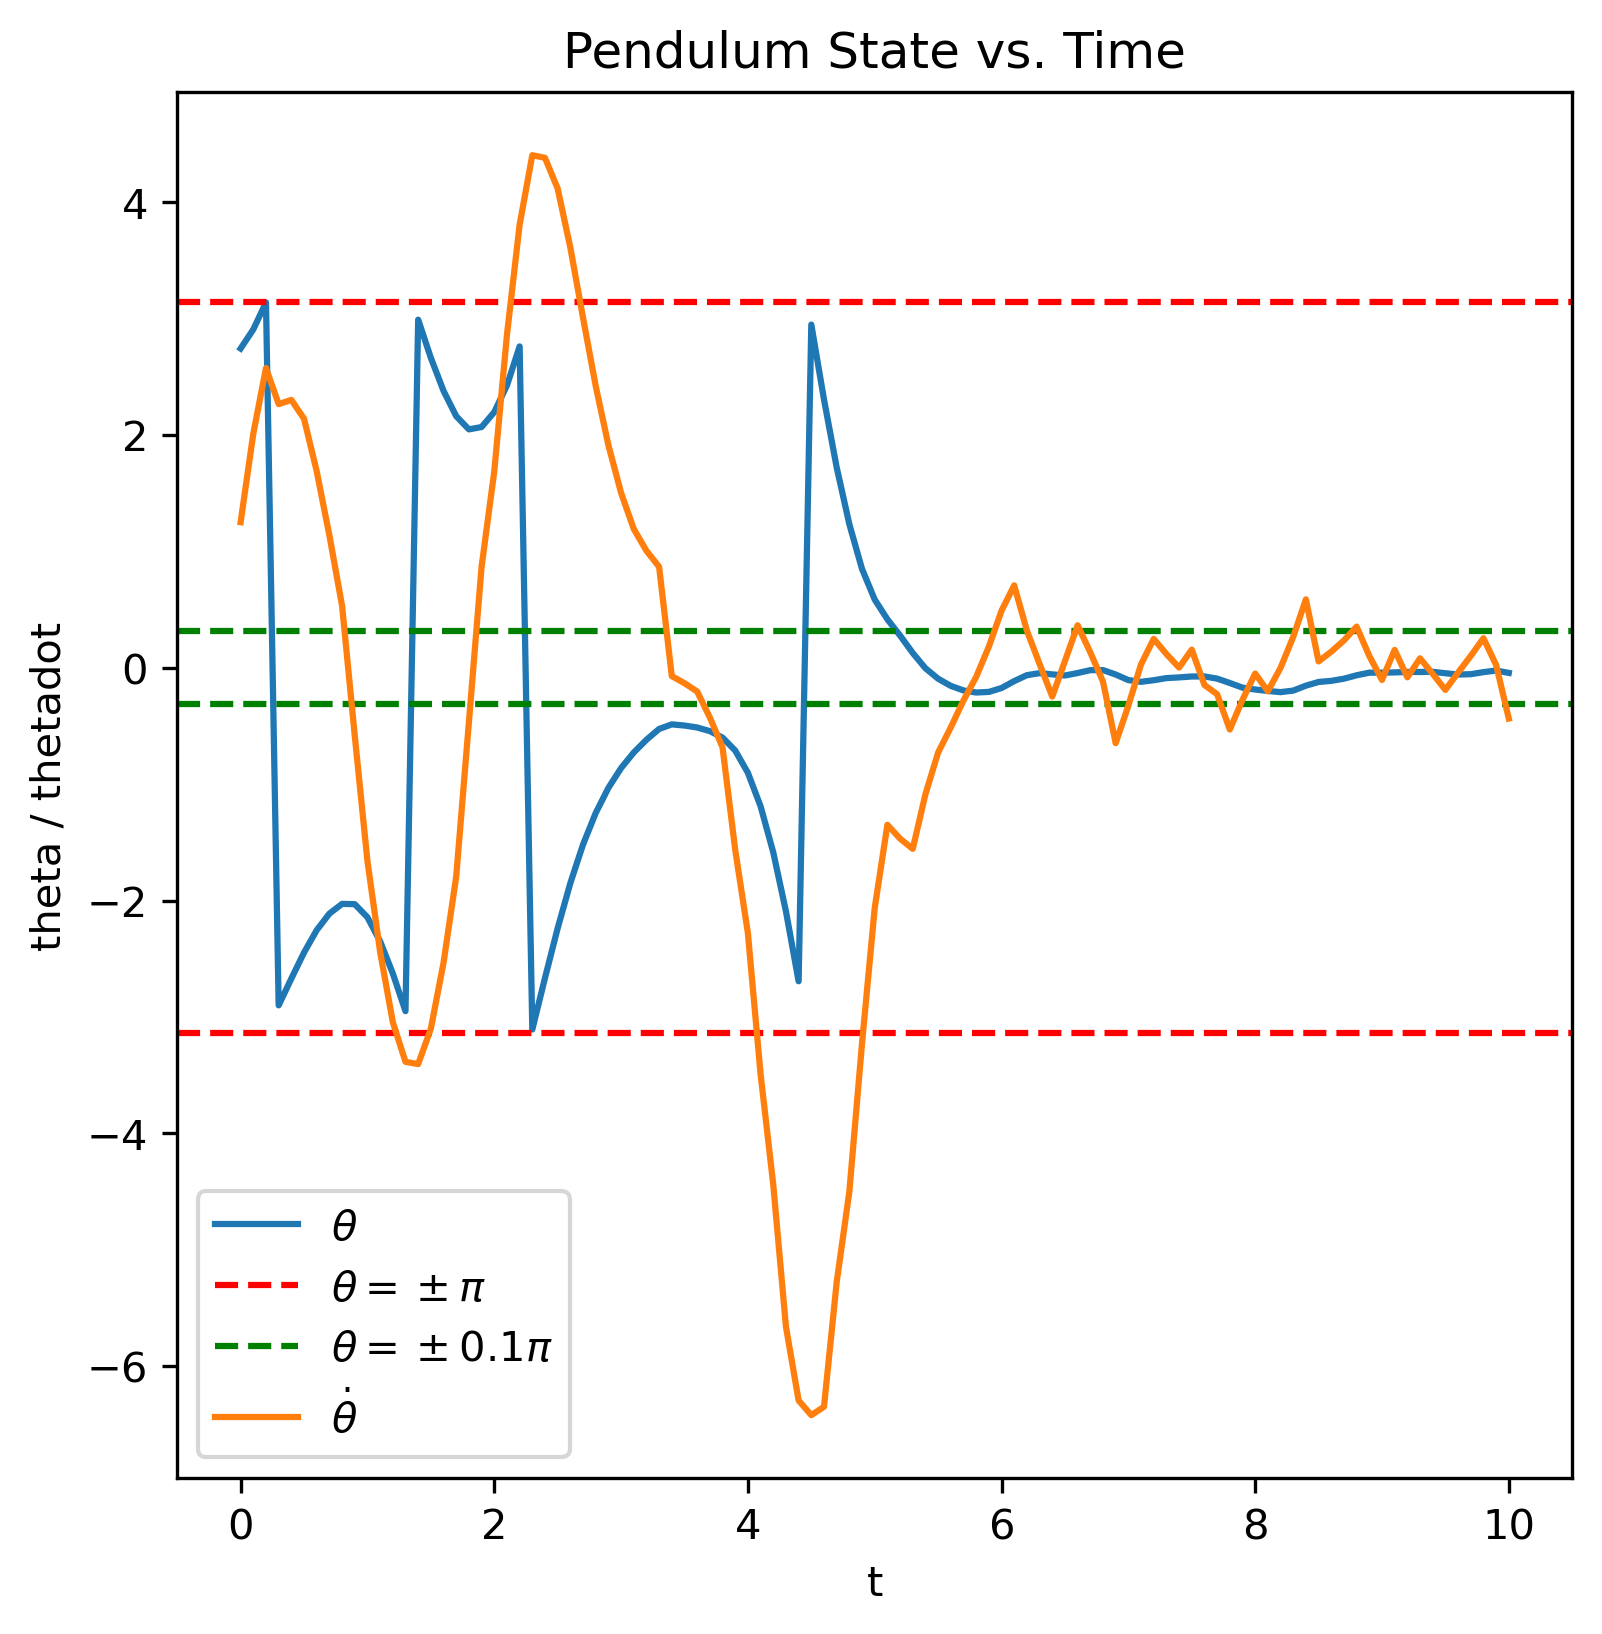
\includegraphics[width=\linewidth]{../figures/yes_target_yes_replay/state_150_1000.png}
\caption{State evolution for the standard DQN algorithm}
\label{fig:yes_target_yes_replay_state_evolution}
\end{figure}
We see that in the example trajectory, the pendulum converges to be within 0.1$\pi$ of vertical at around halfway through the trajectory. There were more scenarios where this convergence was quicker, this trajectory just presents success with one of the worse initial conditions.

\subsection{DQN Algorithm: No Target Network}
The DQN algorithm without a target network was run for 150 episodes. The distinction here was that the target Q network was updated every step to be the same as the Q network. The results are shown in Fig. \ref{fig:no_target_yes_replay_one_run}.

\begin{figure}[h]
\centering
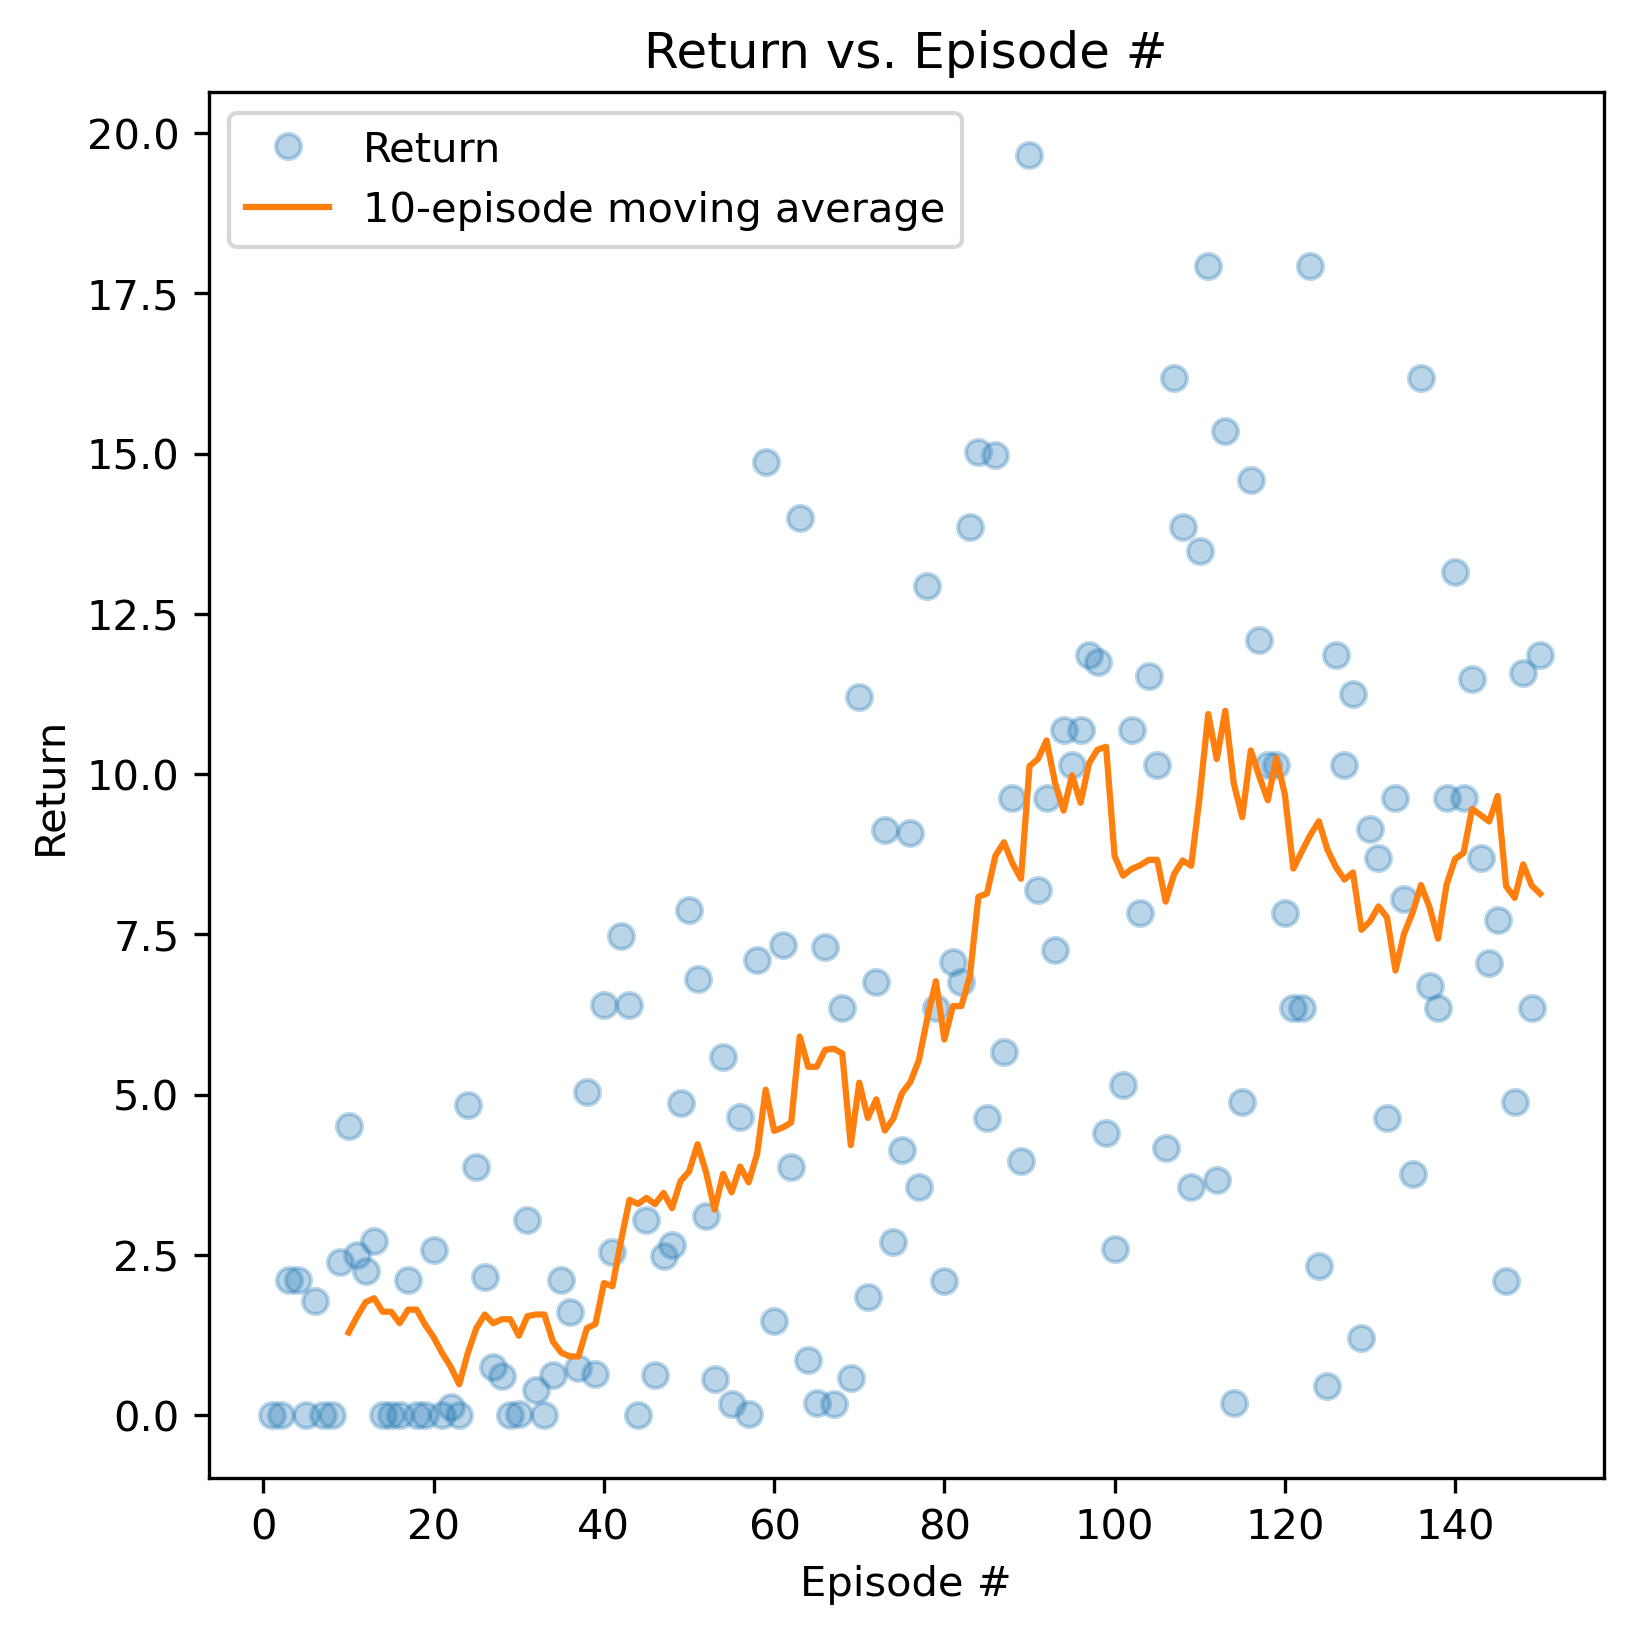
\includegraphics[width=0.87\linewidth]{../figures/no_target_yes_replay/return_150_1.png}
\caption{Learning curve for one run of the DQN algorithm without a target network}
\label{fig:no_target_yes_replay_one_run}
\end{figure}
Similarly to the standard DQN algorithm, the DQN algorithm without a target network was run 10 times and the mean return and 1-sigma bounds are shown in Fig. \ref{fig:no_target_yes_replay_10_runs}.

\begin{figure}[h]
\centering
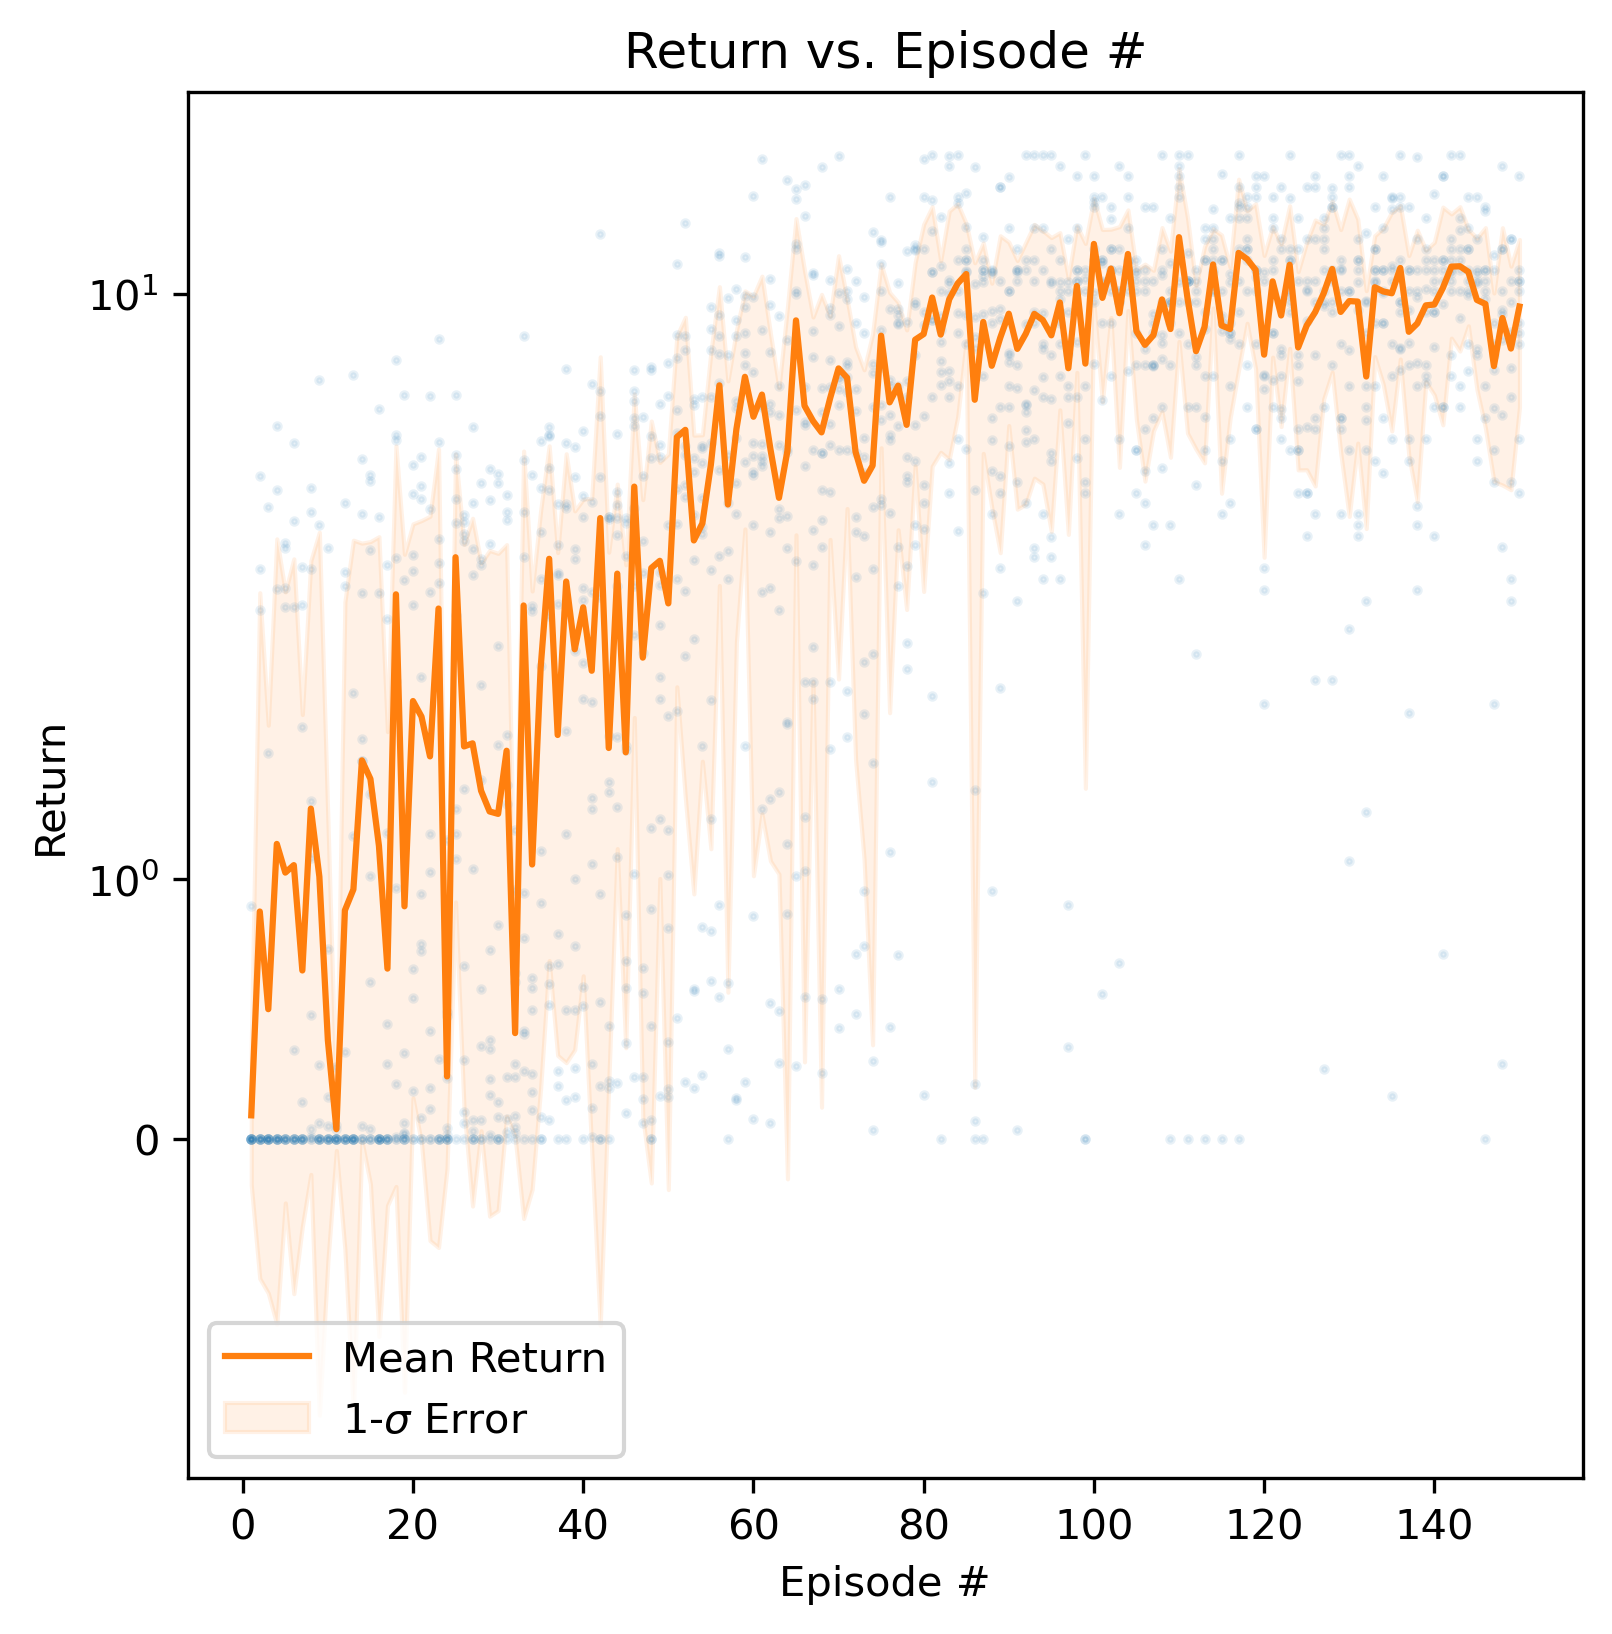
\includegraphics[width=\linewidth]{../figures/no_target_yes_replay/mean_return_150_1_log_True.png}
\caption{Mean return and 1-sigma bounds for 10 runs of the DQN algorithm without a target network}
\label{fig:no_target_yes_replay_10_runs}
\end{figure}
The mean return for the 10-run case is around 10, which is similar to the standard DQN algorithm. Therefore, updating the target network every step does not seem to have a significant impact on the learning curve. The learned policy and value function are shown in Fig. \ref{fig:no_target_yes_replay_policy} and Fig. \ref{fig:no_target_yes_replay_value_function}, respectively.

\begin{figure}[h]
\centering
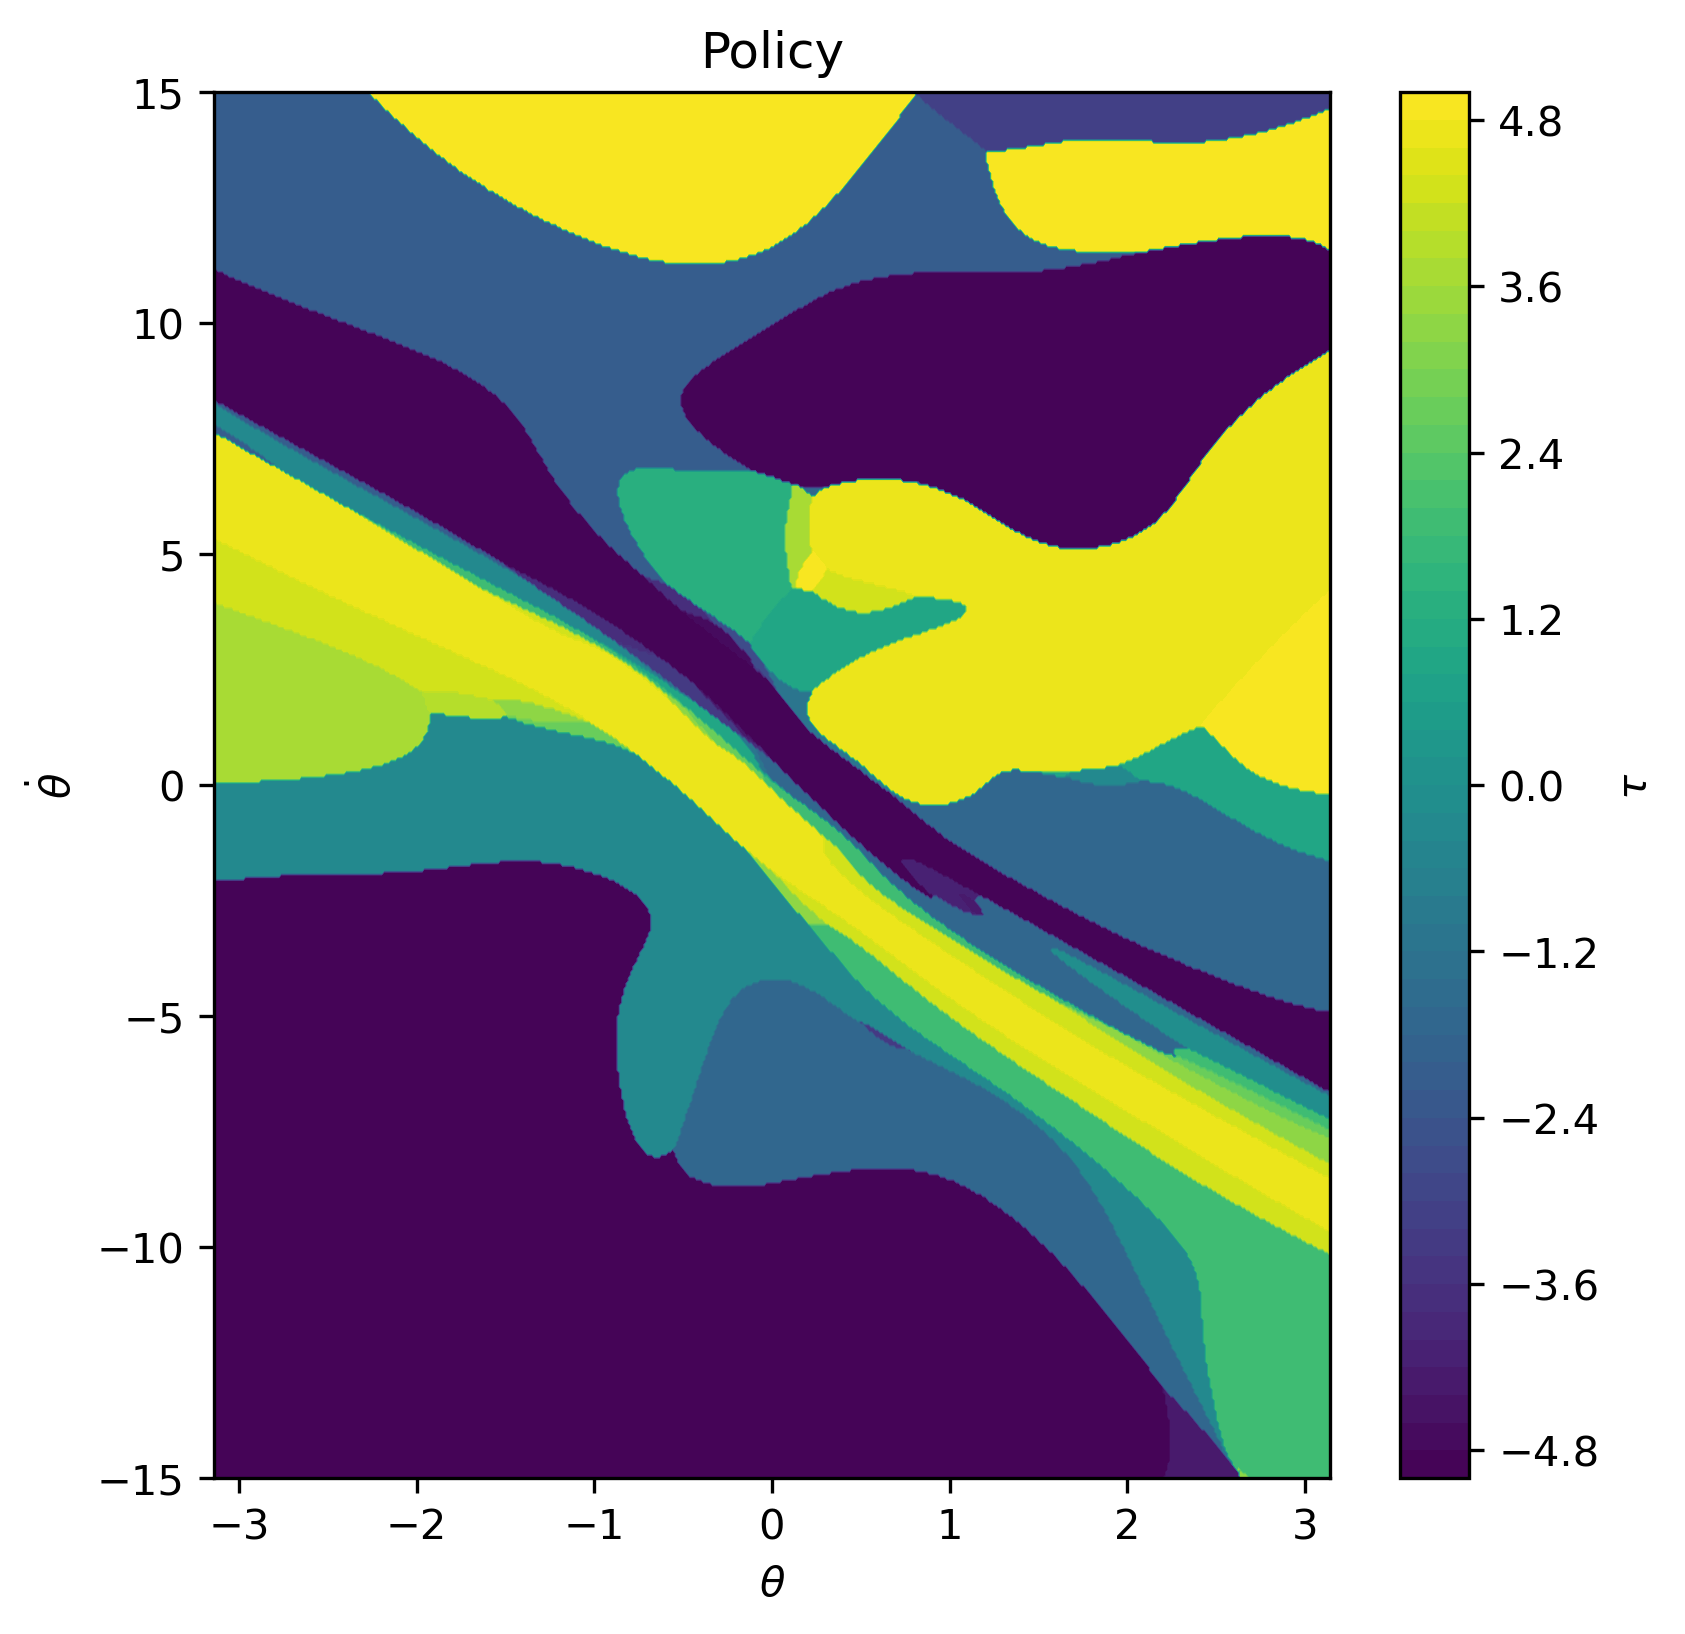
\includegraphics[width=\linewidth]{../figures/no_target_yes_replay/ctr_policy_150_1.png}
\caption{Learned policy for the DQN algorithm without a target network}
\label{fig:no_target_yes_replay_policy}
\end{figure}
\begin{figure}[h]
\centering
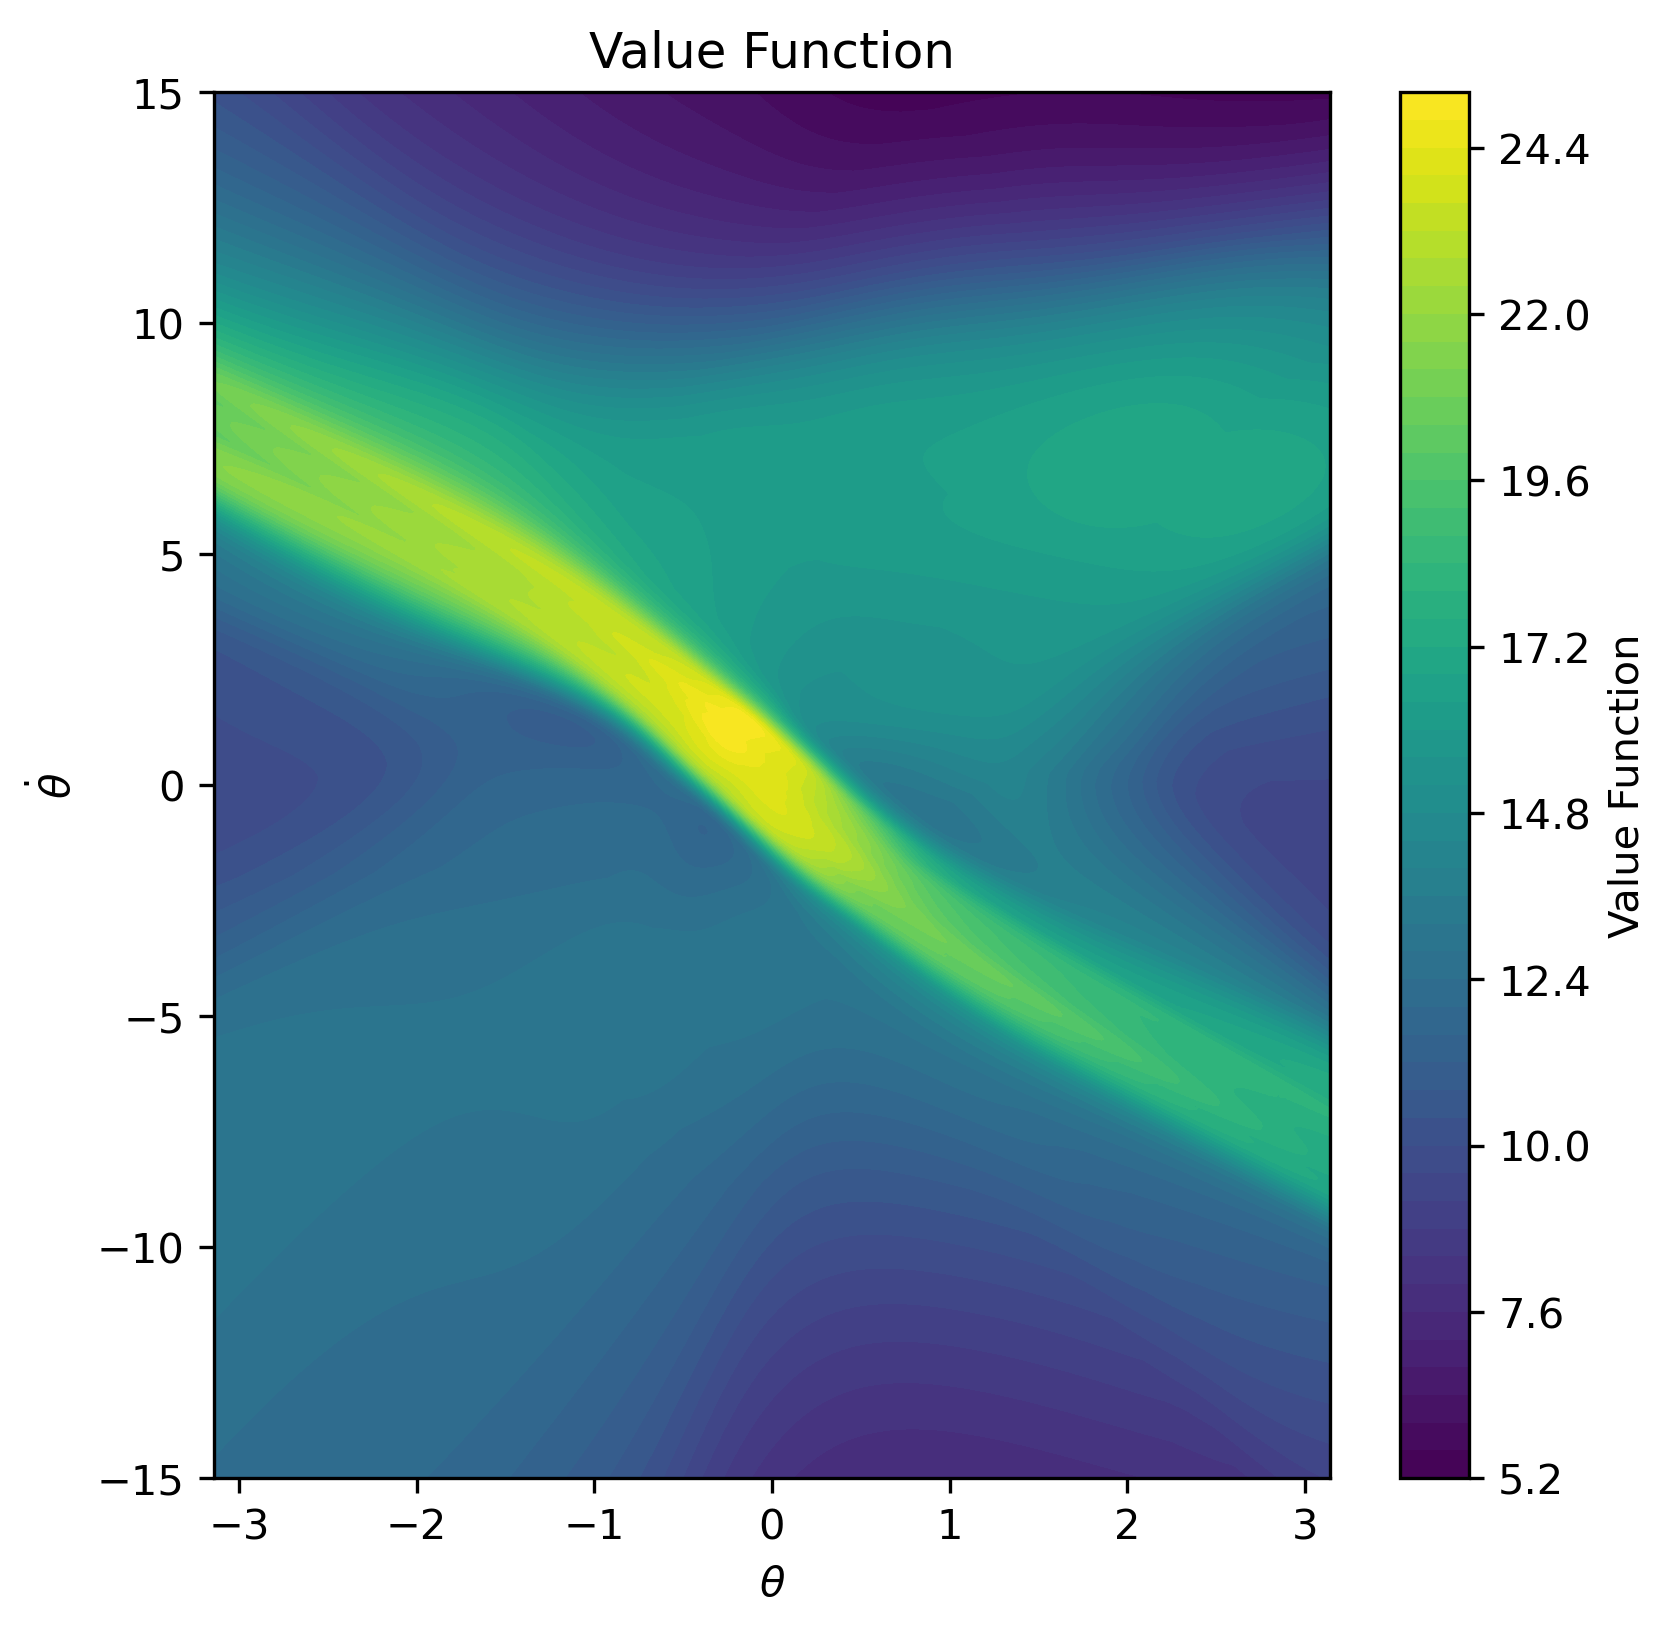
\includegraphics[width=\linewidth]{../figures/no_target_yes_replay/ctr_value_func_150_1.png}
\caption{Value function for the DQN algorithm without a target network}
\label{fig:no_target_yes_replay_value_function}
\end{figure}

\newpage
\subsection{DQN Algorithm: No Experience Replay}
The DQN algorithm without experience replay was also run for 150 episodes. In the case of no experience replay, the minibatch is not sampled from the replay buffer, but rather from the most recent transitions. In this case, the target network was updated every 1000 steps (same as the standard DQN algorithm). The results from a single run are shown in Fig. \ref{fig:yes_target_no_replay_one_run} and the result from 10 runs are shown in Fig. \ref{fig:yes_target_no_replay_10_runs}.

\begin{figure}[h]
\centering
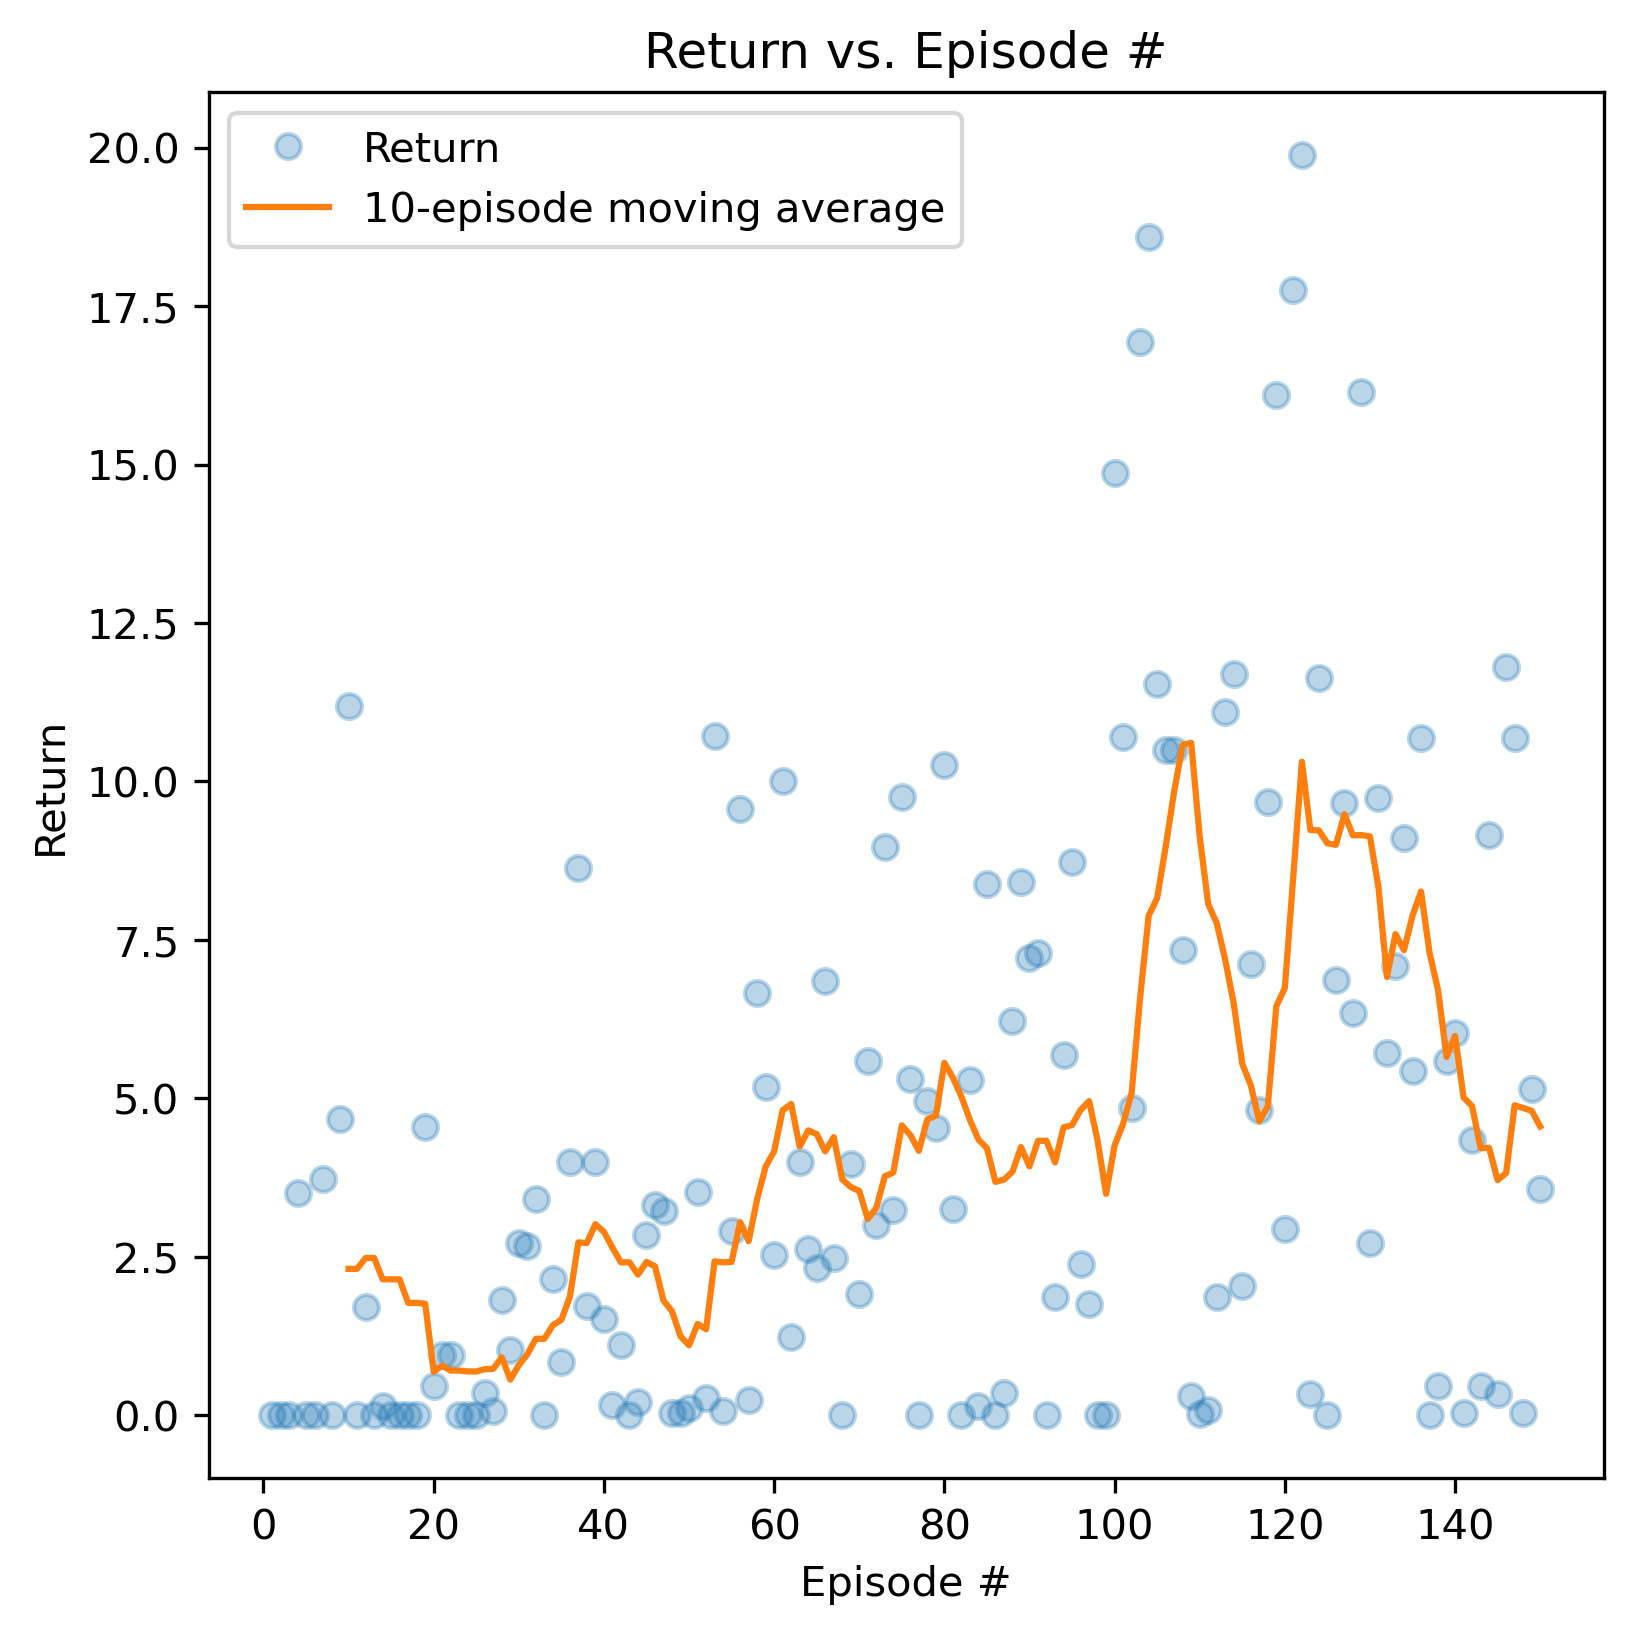
\includegraphics[width=0.94\linewidth]{../figures/yes_target_no_replay/return_150_1000.png}
\caption{Learning curve for one run of the DQN algorithm without experience replay}
\label{fig:yes_target_no_replay_one_run}
\end{figure}
\begin{figure}[h]
\centering
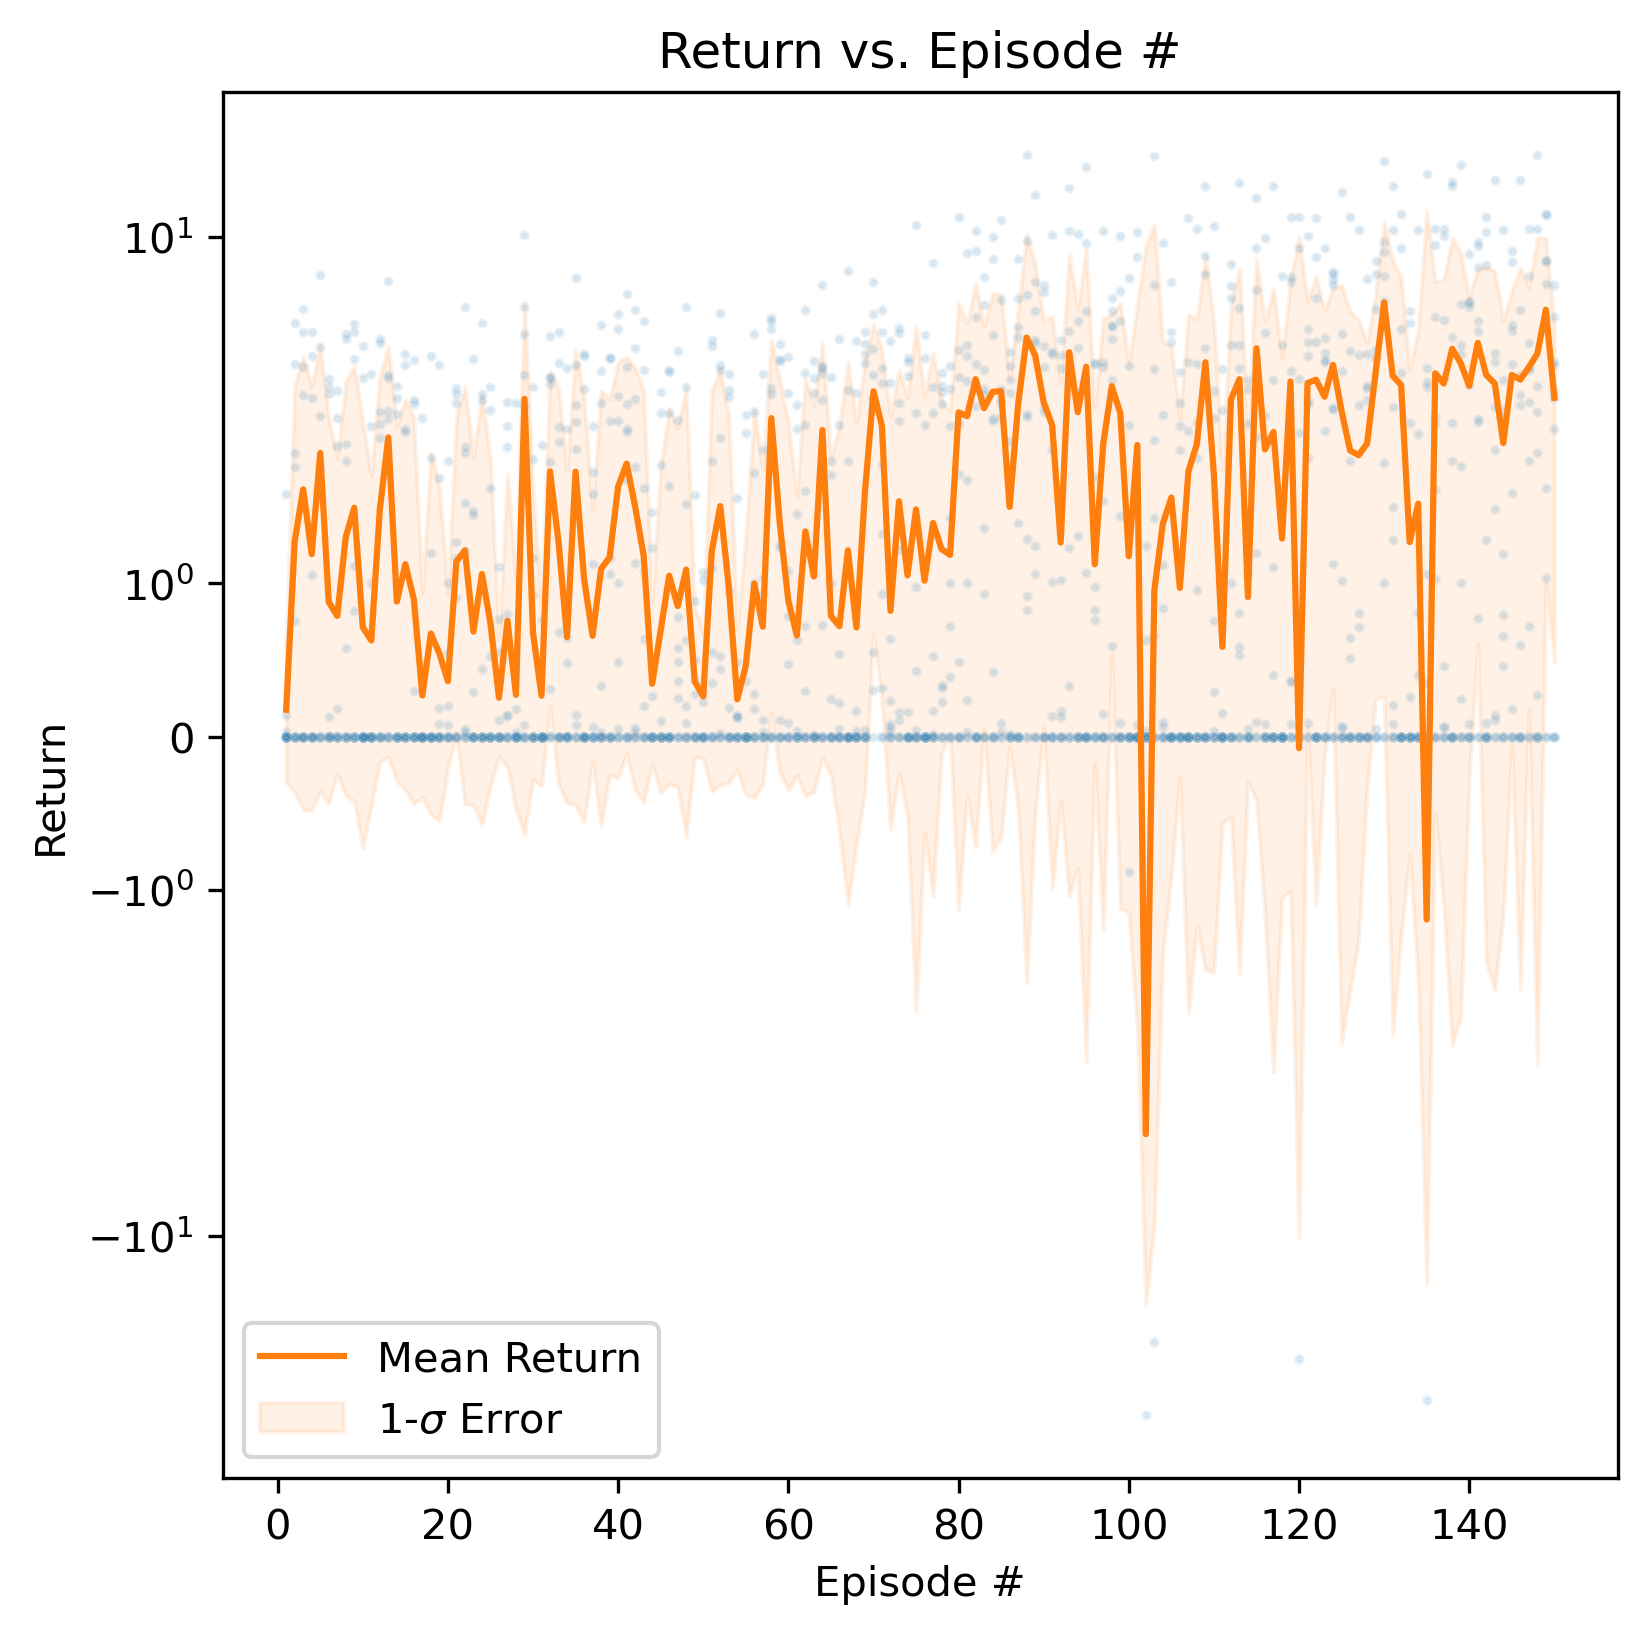
\includegraphics[width=0.95\linewidth]{../figures/yes_target_no_replay/mean_return_150_1000_log_True.png}
\caption{Mean return and 1-sigma bounds for 10 runs of the DQN algorithm without experience replay}
\label{fig:yes_target_no_replay_10_runs}
\end{figure}
The mean return in this case is lower compared to the standard DQN algorithm or the standard DQN algorithm without a target network. This indicates that the experience replay is a significant factor in the learning process. Additionally, the experience replay seems to help with remembering the optimal policy, since without it the reward has canstant peaks and valleys. The learned policy and value function are shown in Fig. \ref{fig:yes_target_no_replay_policy} and Fig. \ref{fig:yes_target_no_replay_value_function}, respectively.

\begin{figure}[h]
\centering
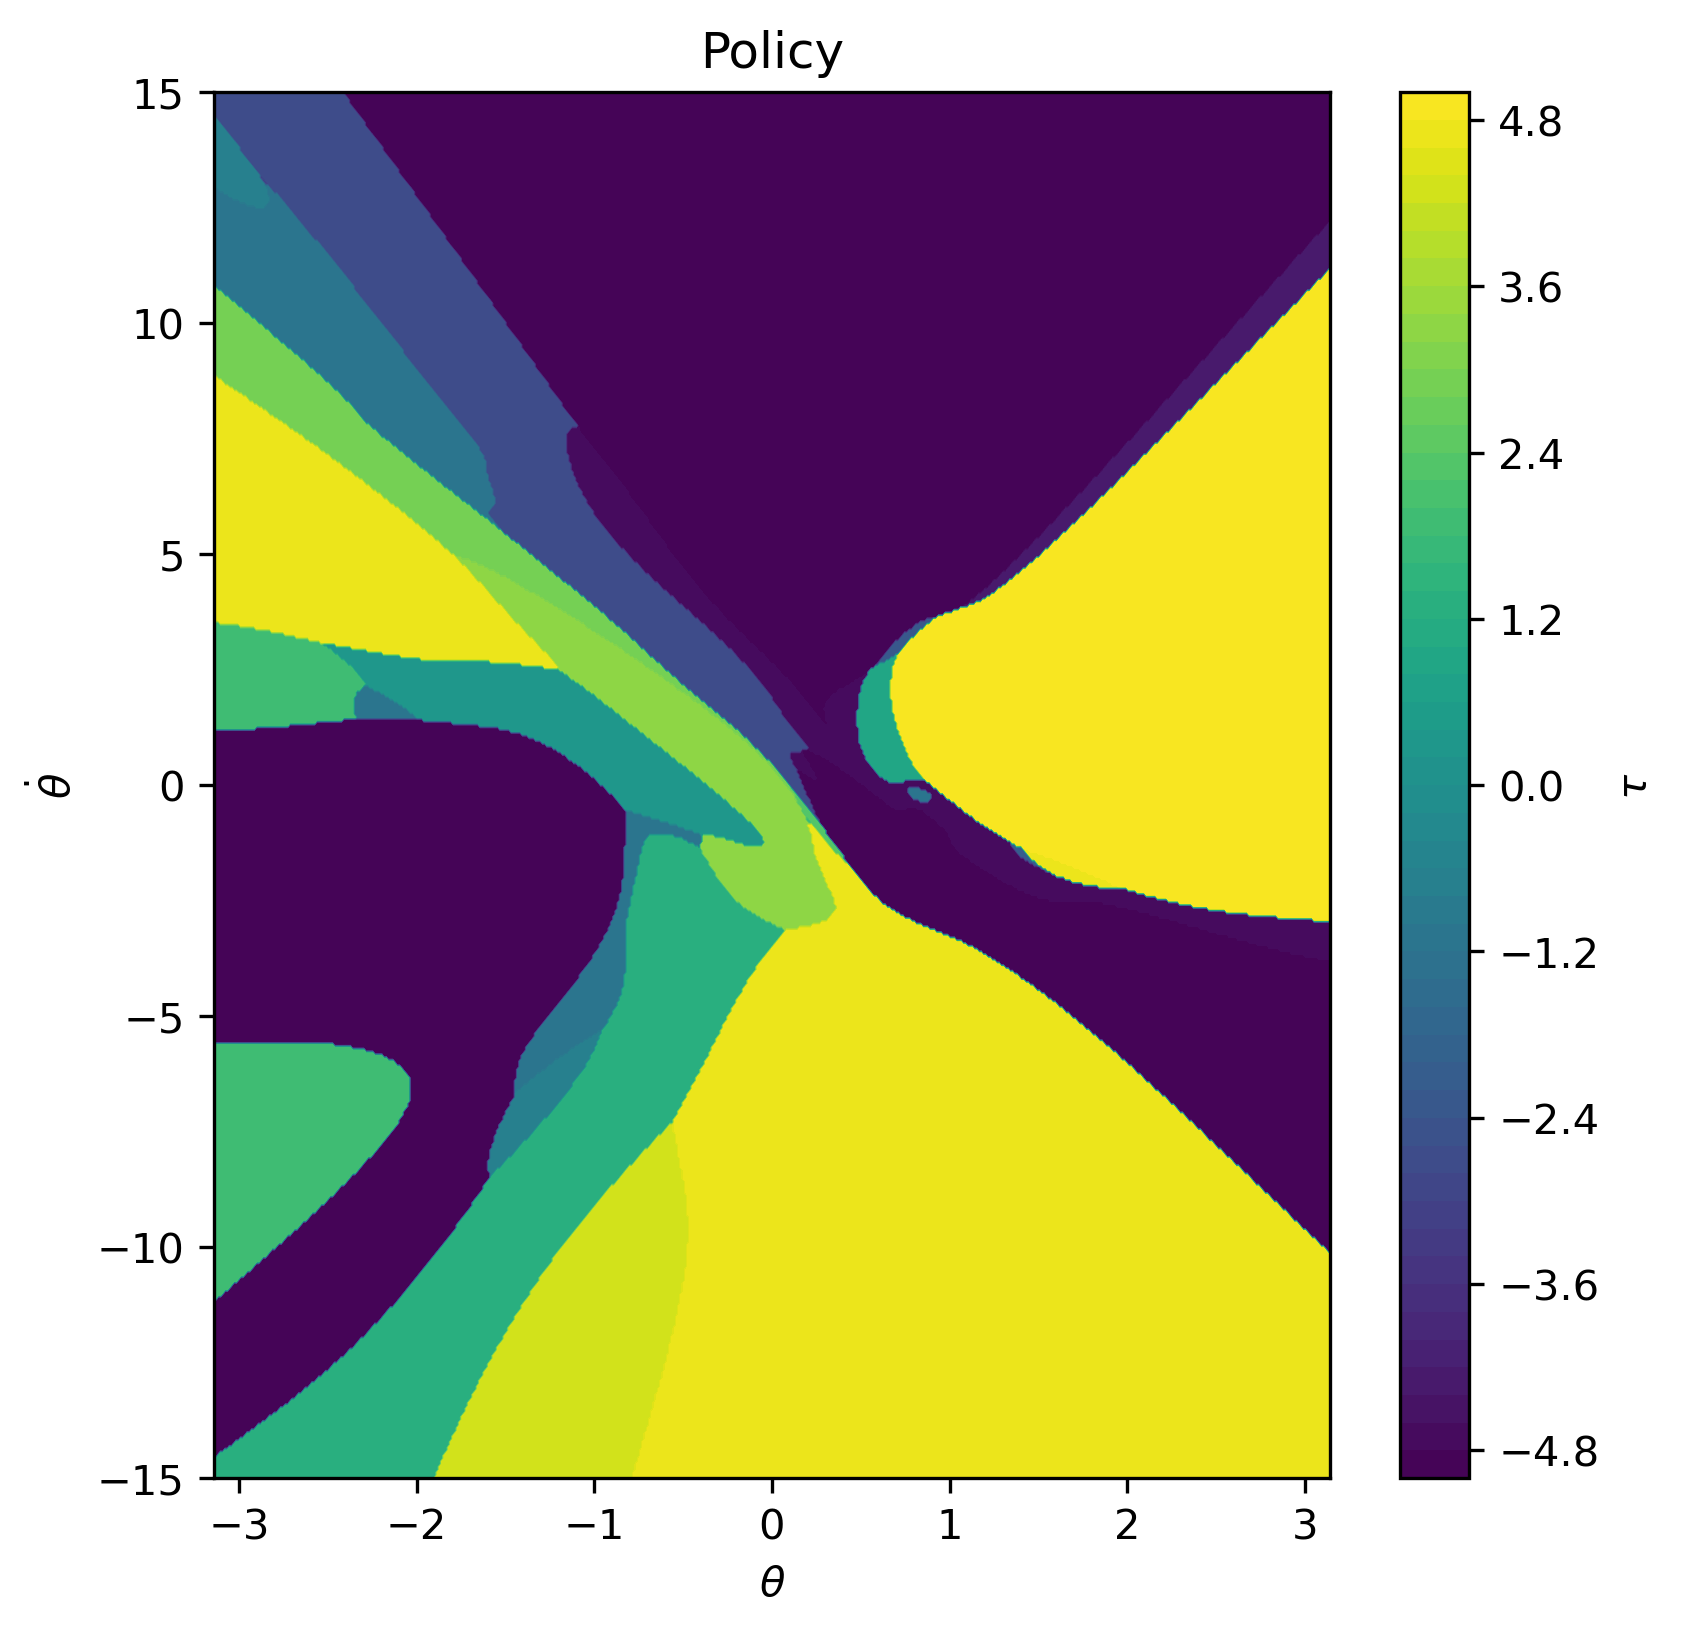
\includegraphics[width=\linewidth]{../figures/yes_target_no_replay/ctr_policy_150_1000.png}
\caption{Learned policy for the DQN algorithm without experience replay}
\label{fig:yes_target_no_replay_policy}
\end{figure}
\begin{figure}[h]
\centering
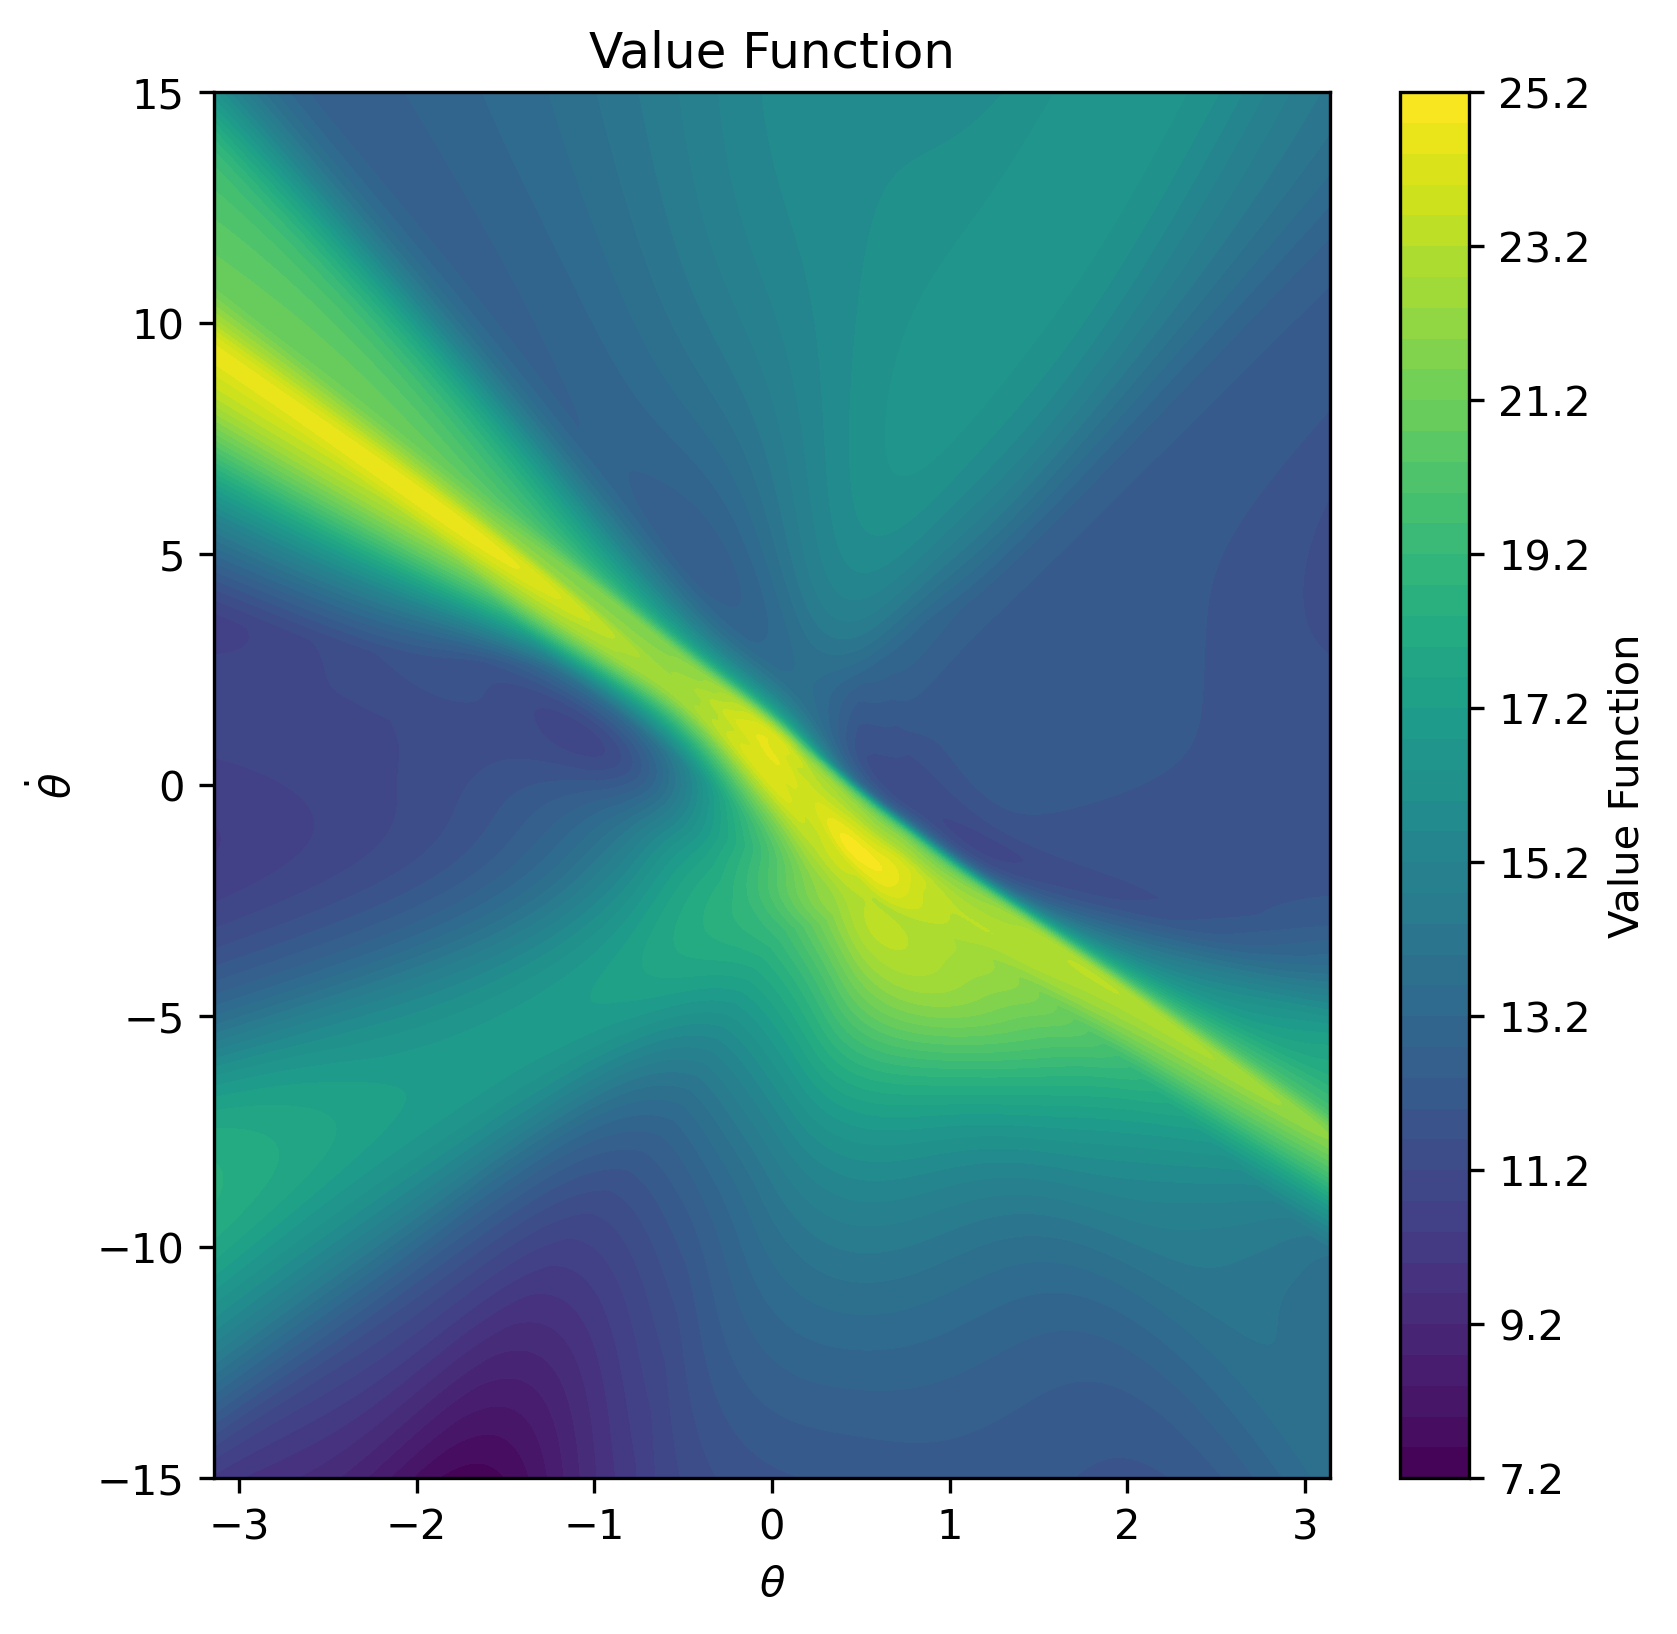
\includegraphics[width=\linewidth]{../figures/yes_target_no_replay/ctr_value_func_150_1000.png}
\caption{Value function for the DQN algorithm without experience replay}
\label{fig:yes_target_no_replay_value_function}
\end{figure}

\subsection{DQN Algorithm: No Experience Replay or Target Network}
The DQN algorithm without experience replay and target network was also run for 150 episodes, just like every previous case. This time, the algorithm has no experience replay or a target network. This means that the target network is the same as the Q network and the minibatch is not sampled from the replay buffer. The results from a single run are shown in Fig. \ref{fig:no_target_no_replay_one_run} and the results from 10 runs are shown in Fig. \ref{fig:no_target_no_replay_10_runs}..

\begin{figure}[h]
\centering
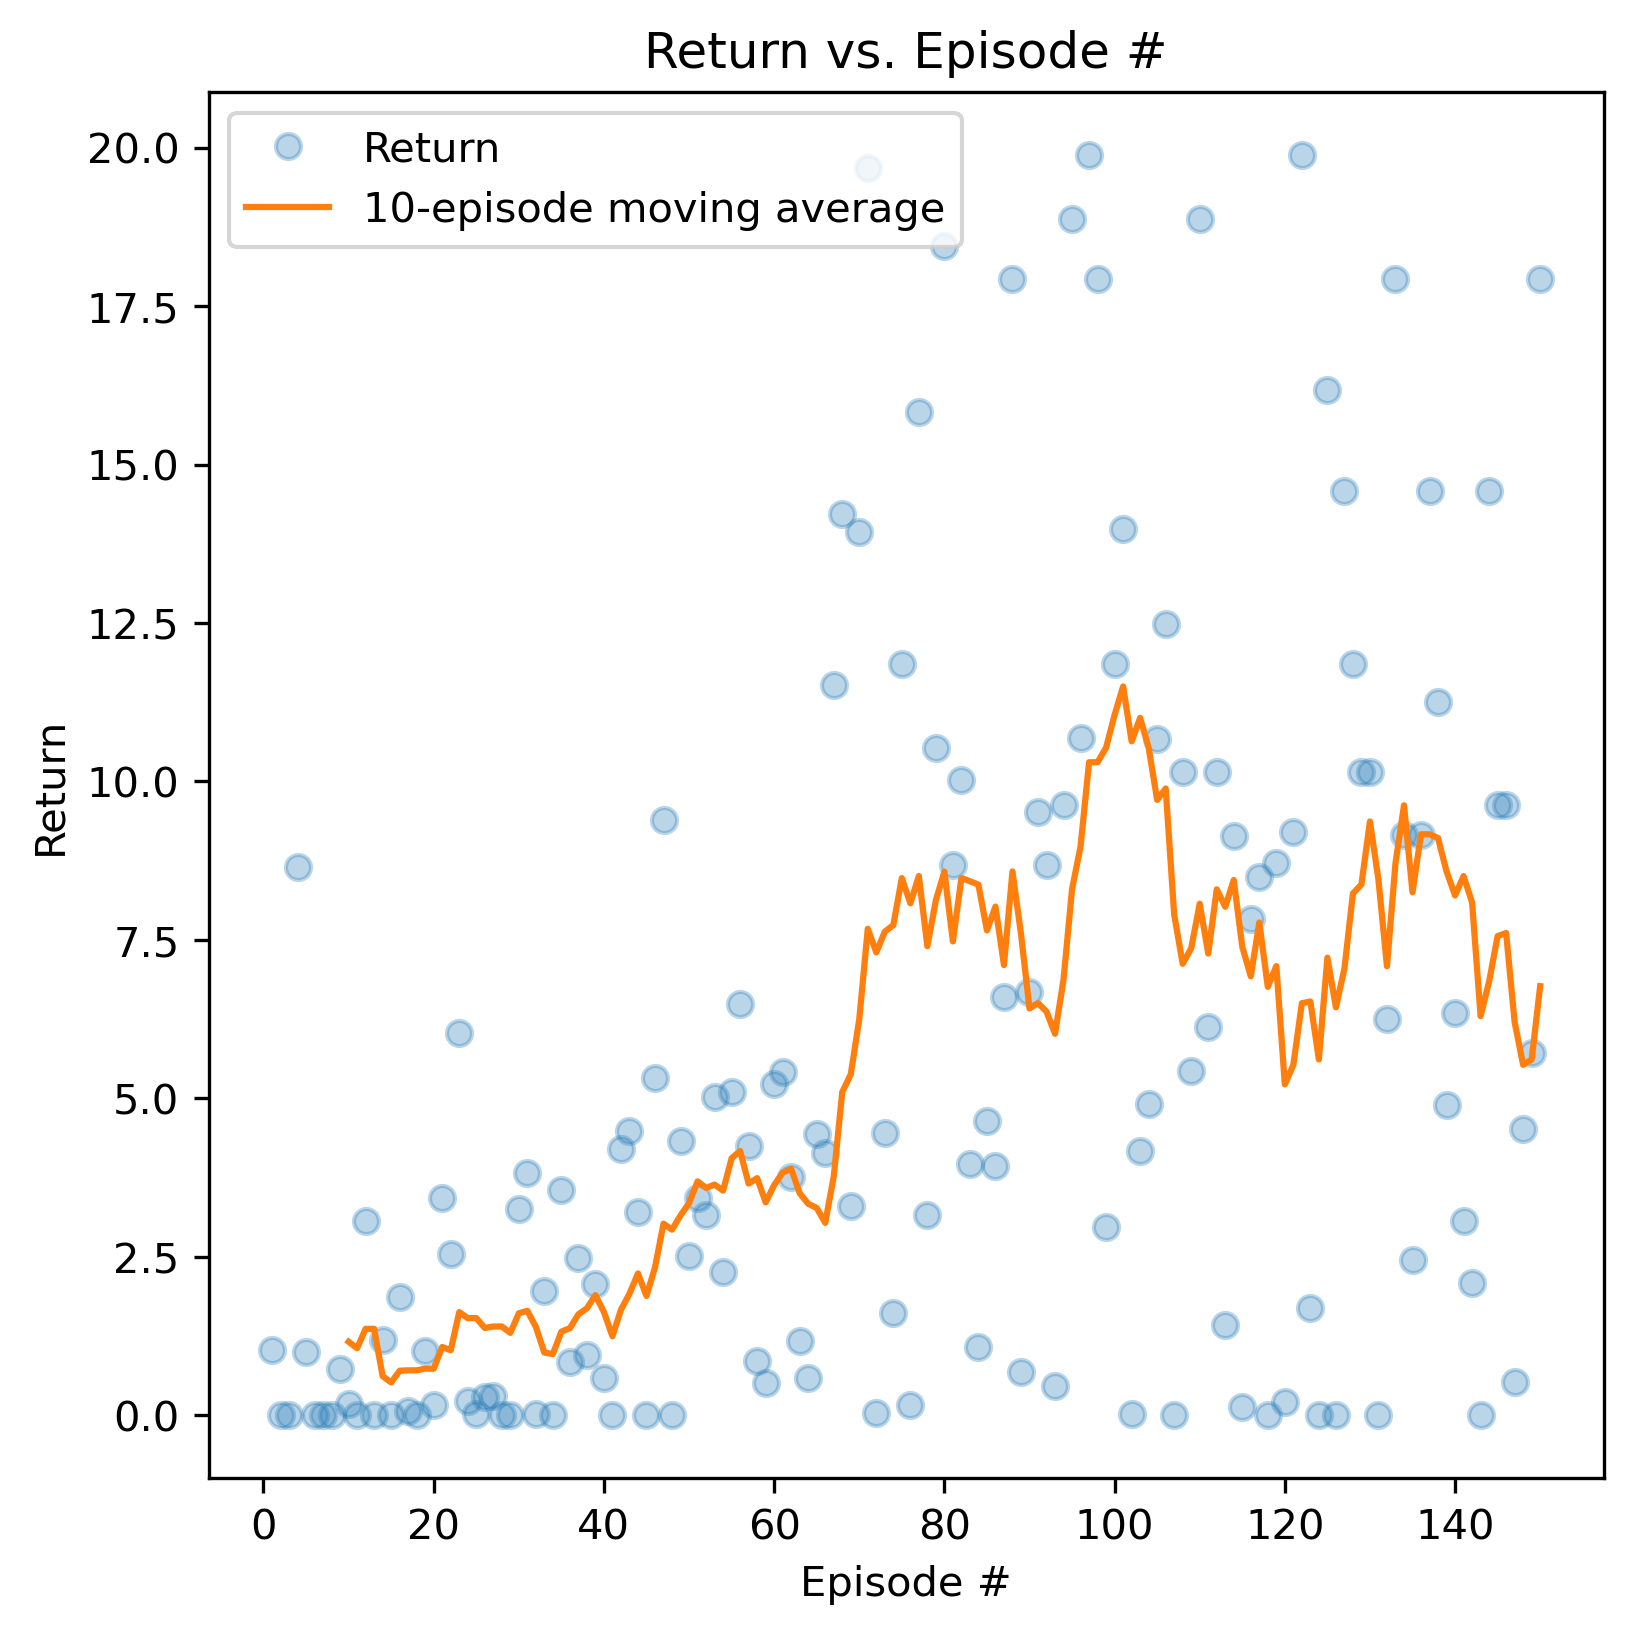
\includegraphics[width=0.94\linewidth]{../figures/no_target_no_replay/return_150_1.png}
\caption{Learning curve for one run of the DQN algorithm without experience replay and target network}
\label{fig:no_target_no_replay_one_run}
\end{figure}
\begin{figure}[h]
\centering
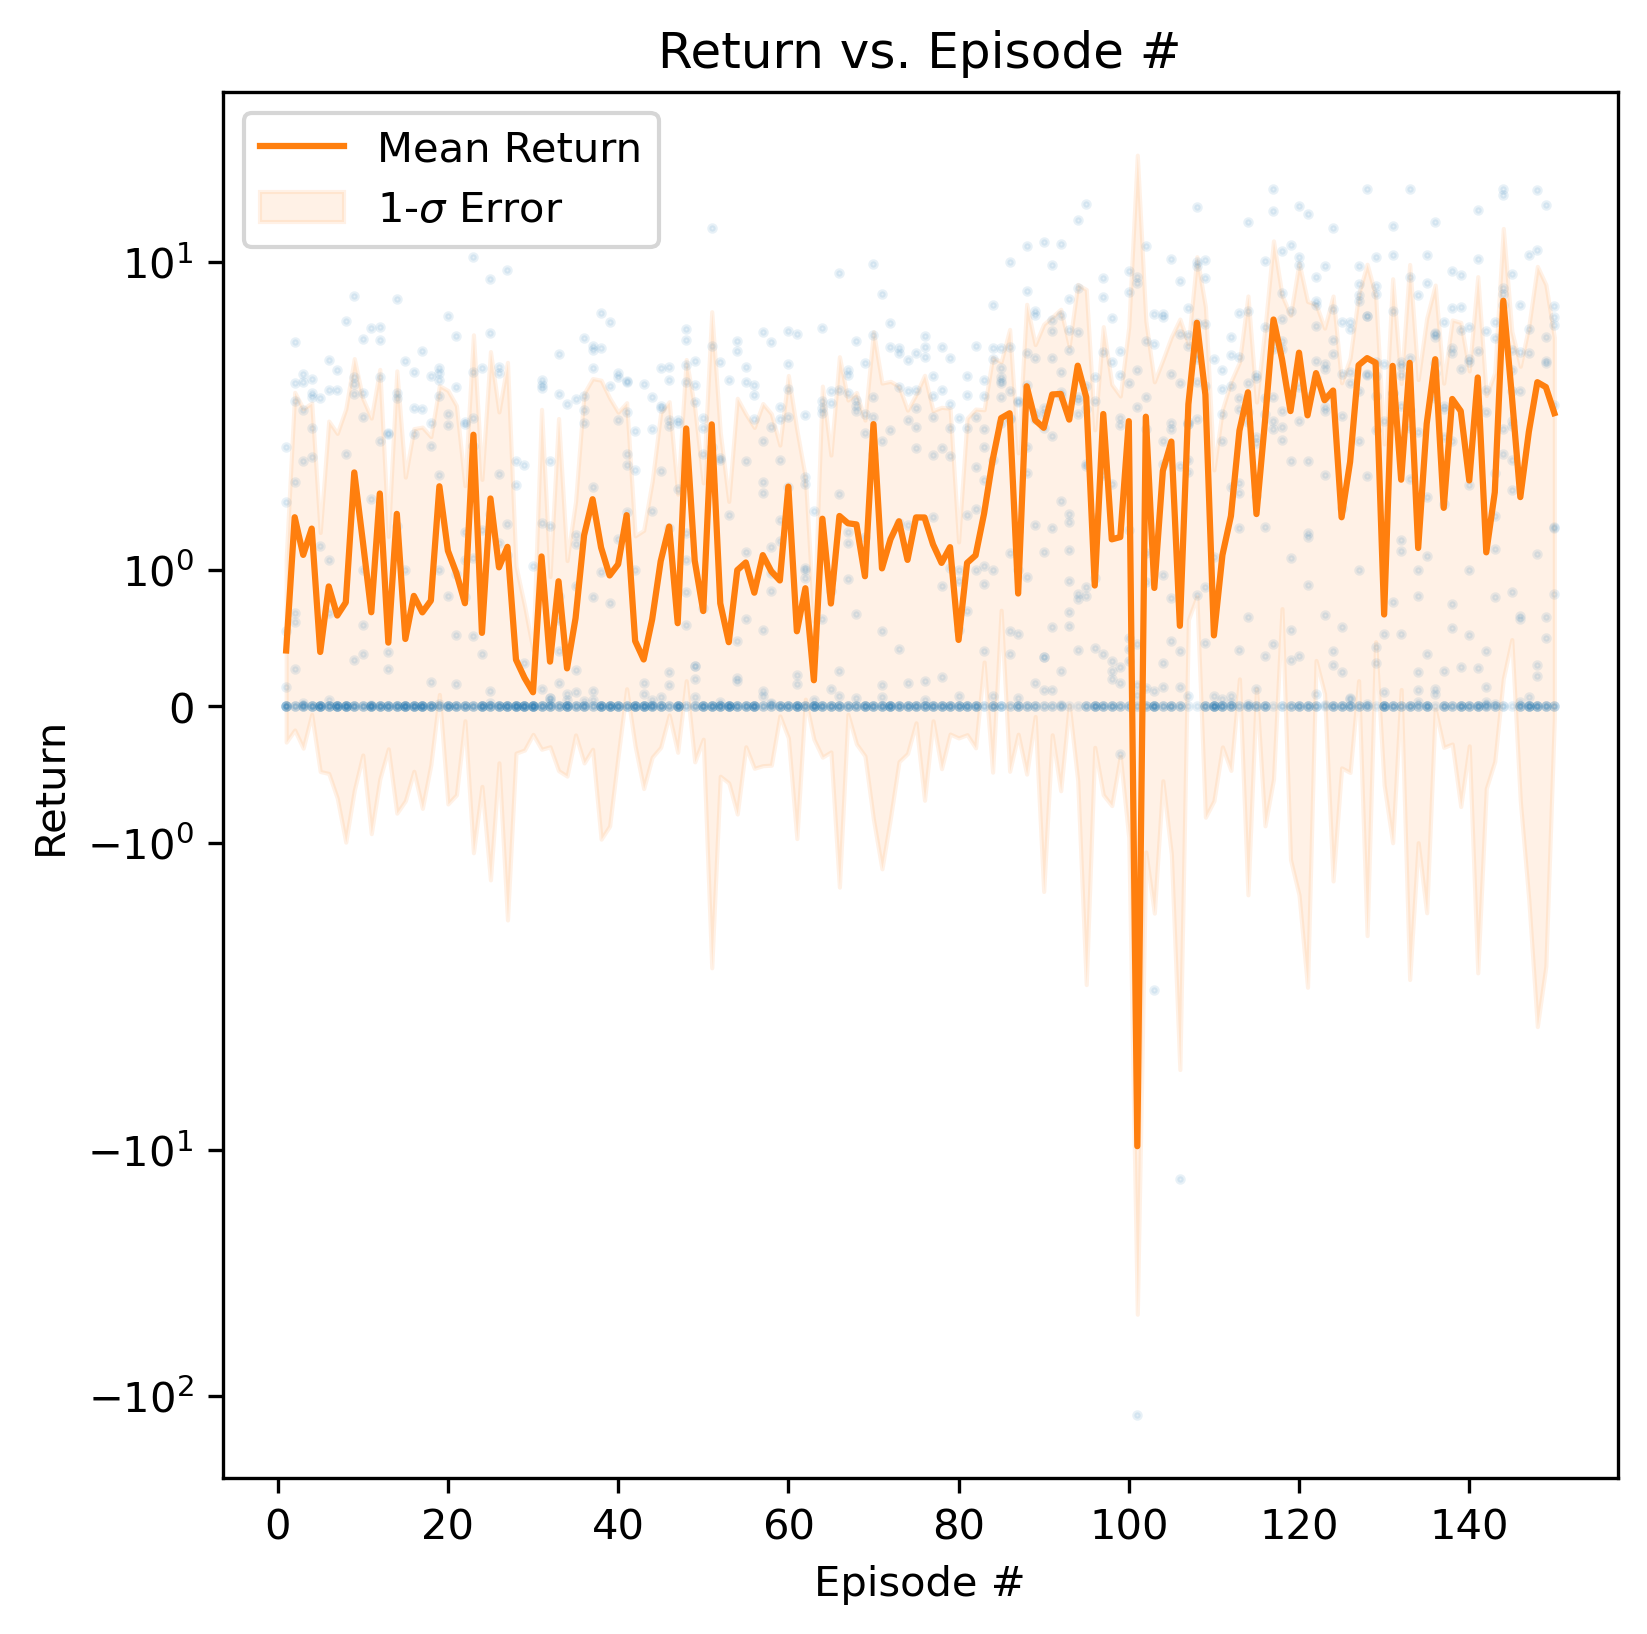
\includegraphics[width=0.95\linewidth]{../figures/no_target_no_replay/mean_return_150_1_log_True.png}
\caption{Mean return and 1-sigma bounds for 10 runs of the DQN algorithm without experience replay and target network}
\label{fig:no_target_no_replay_10_runs}
\end{figure}
The mean return in this case is once again lower than the standard DQN algorithm or the DQN algorithm without target network. However, it is similar to the DQN algorithm without experience replay. This once again indicates that the experience replay is a bigger contributor to the learning process than the target network. The learned policy and value function are shown in Fig. \ref{fig:no_target_no_replay_policy} and Fig. \ref{fig:no_target_no_replay_value_function}, respectively.

\begin{figure}[h]
\centering
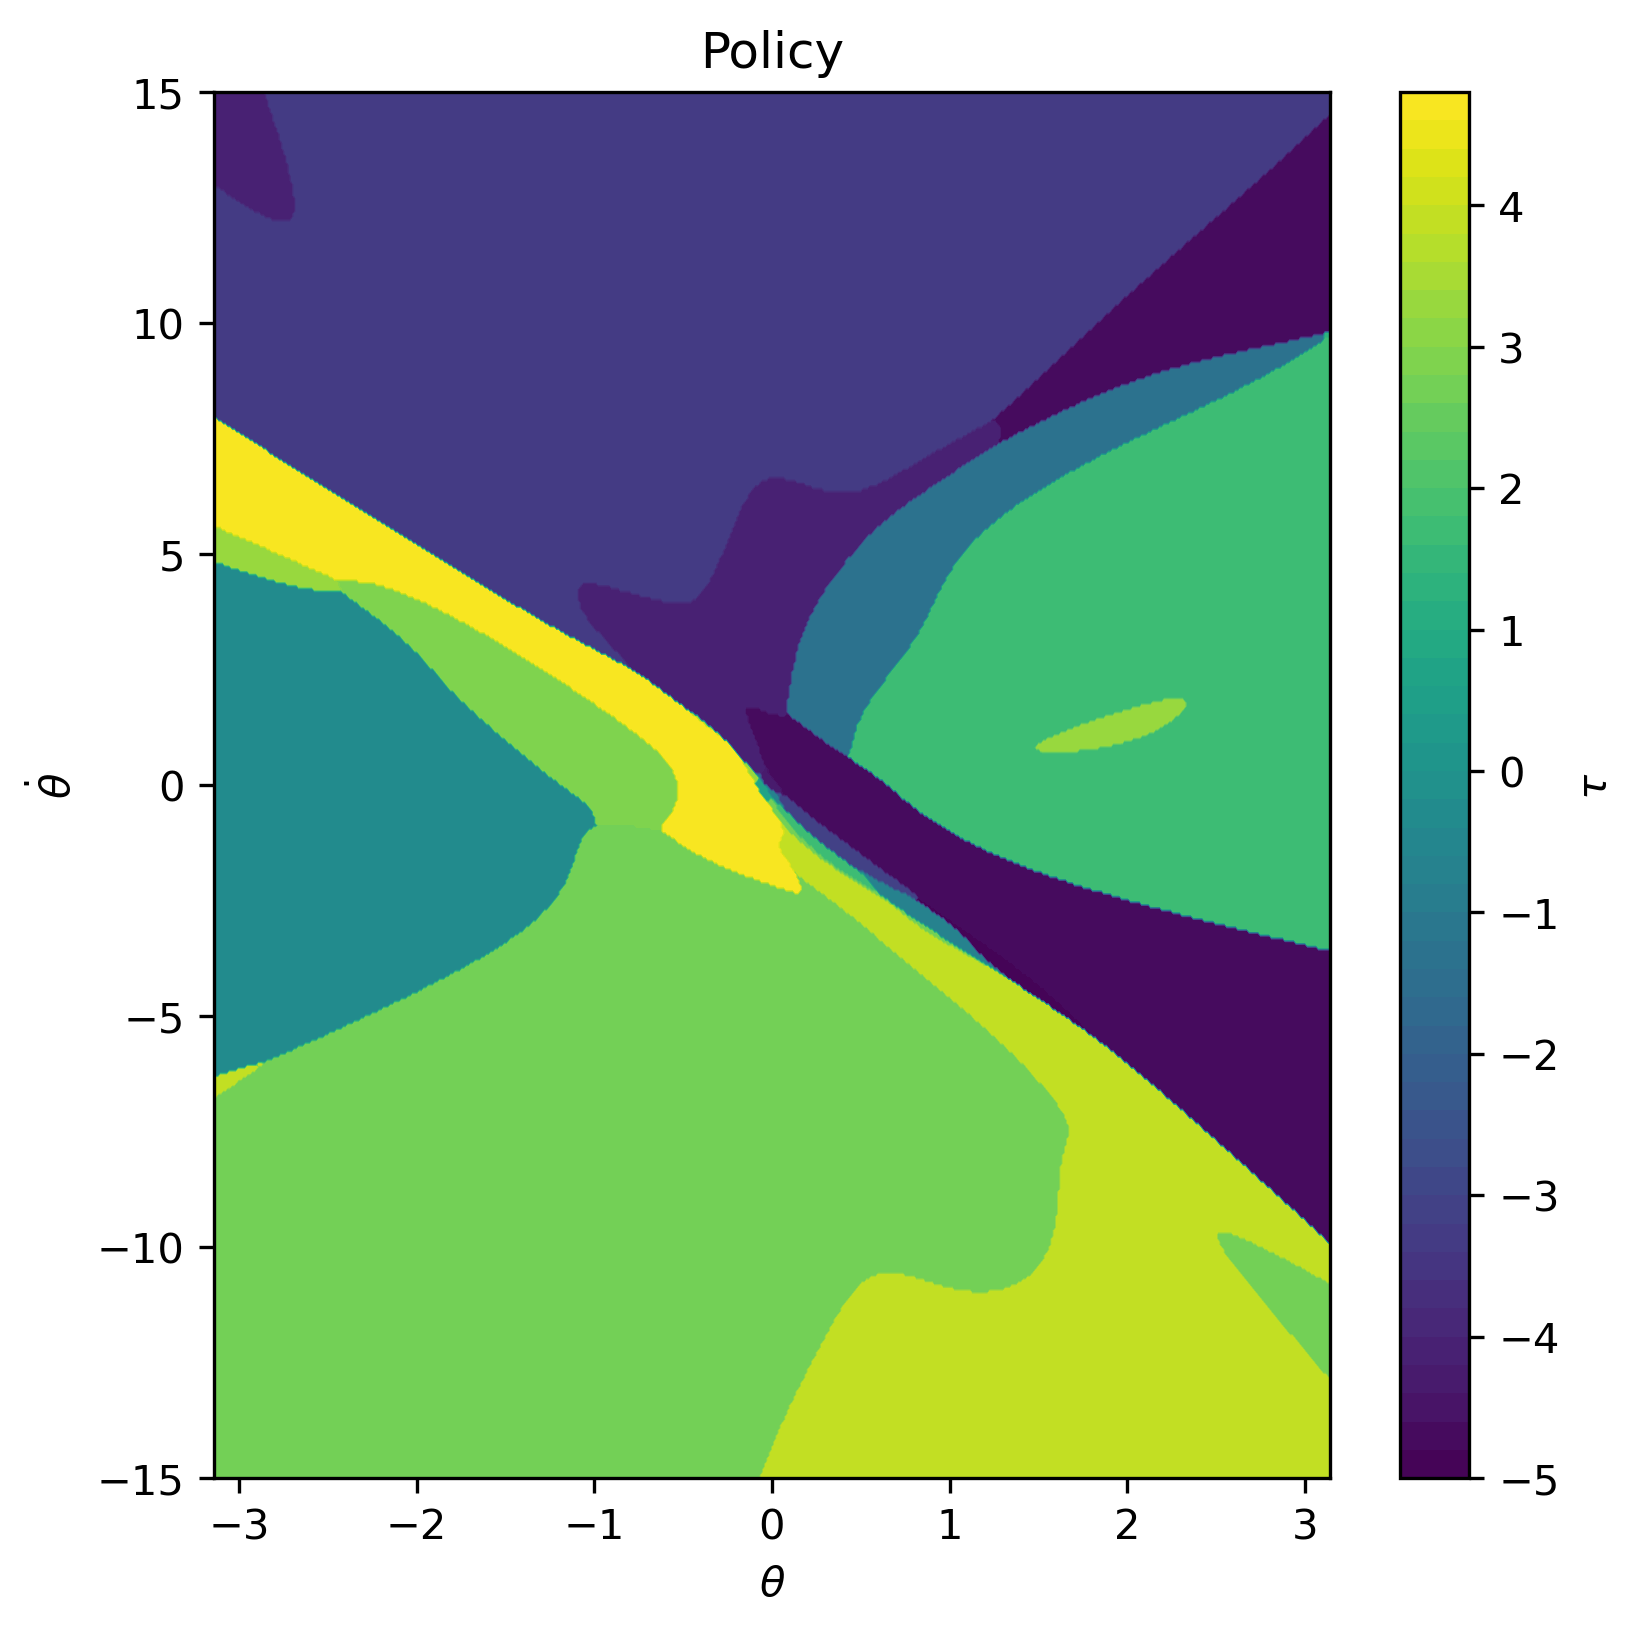
\includegraphics[width=0.98\linewidth]{../figures/no_target_no_replay/ctr_policy_150_1.png}
\caption{Learned policy for the DQN algorithm without experience replay and target network}
\label{fig:no_target_no_replay_policy}
\end{figure}
\begin{figure}[h]
\centering
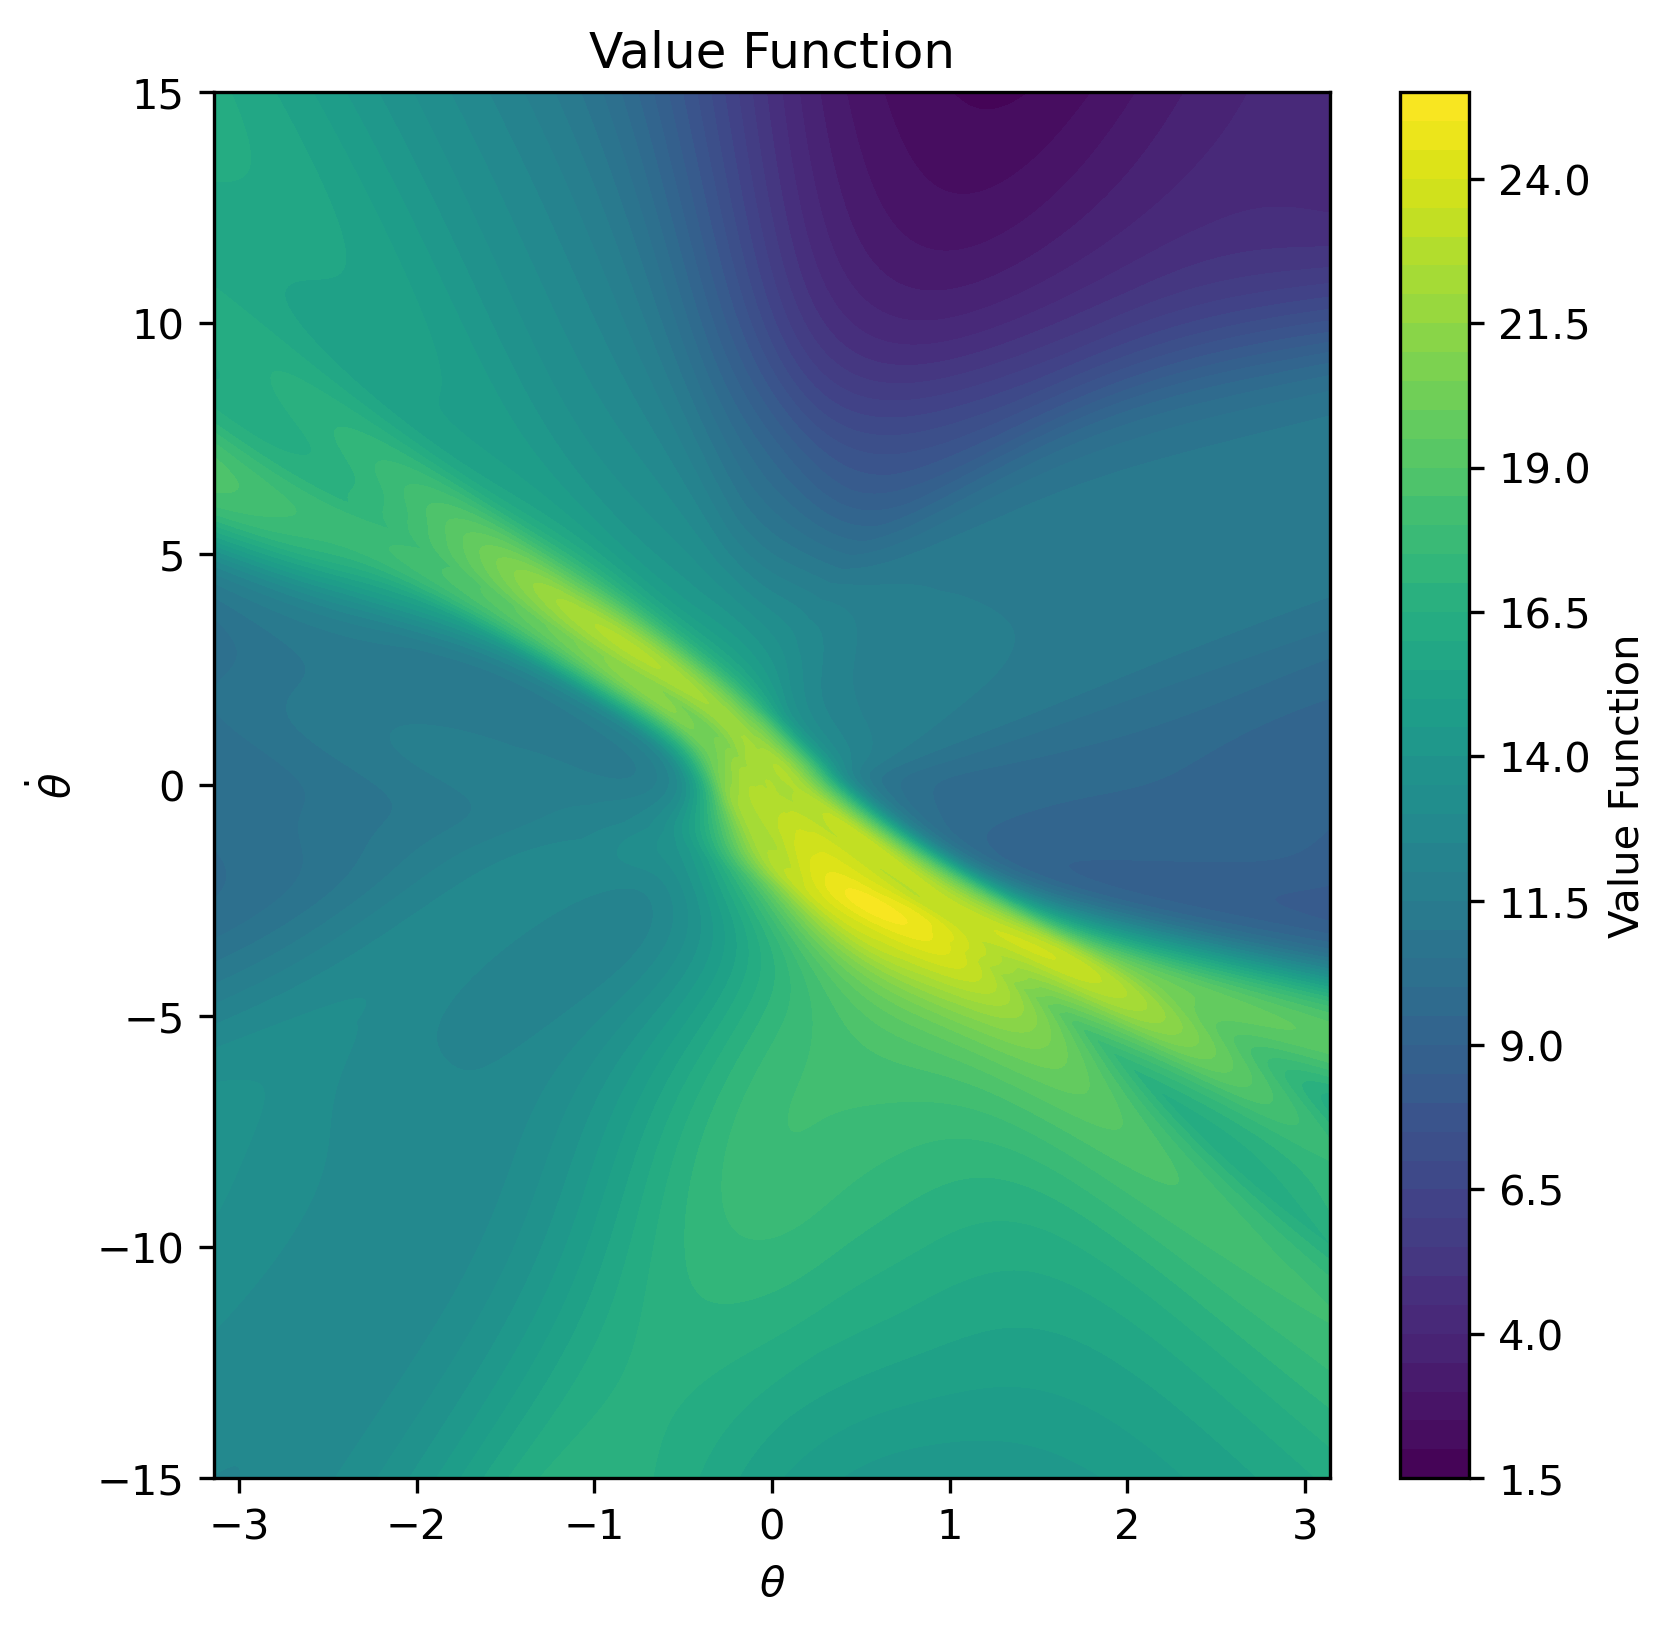
\includegraphics[width=0.99\linewidth]{../figures/no_target_no_replay/ctr_value_func_150_1.png}
\caption{Value function for the DQN algorithm without experience replay and target network}
\label{fig:no_target_no_replay_value_function}
\end{figure}

\subsection{Ablation Study}
Four different flavors of the DQN algorithm were used in this work. The mean return of each algorithm is shown in Fig. \ref{fig:ablation_study_log} and Fig. \ref{fig:ablation_study_linear}.

\begin{figure}[h]
\centering
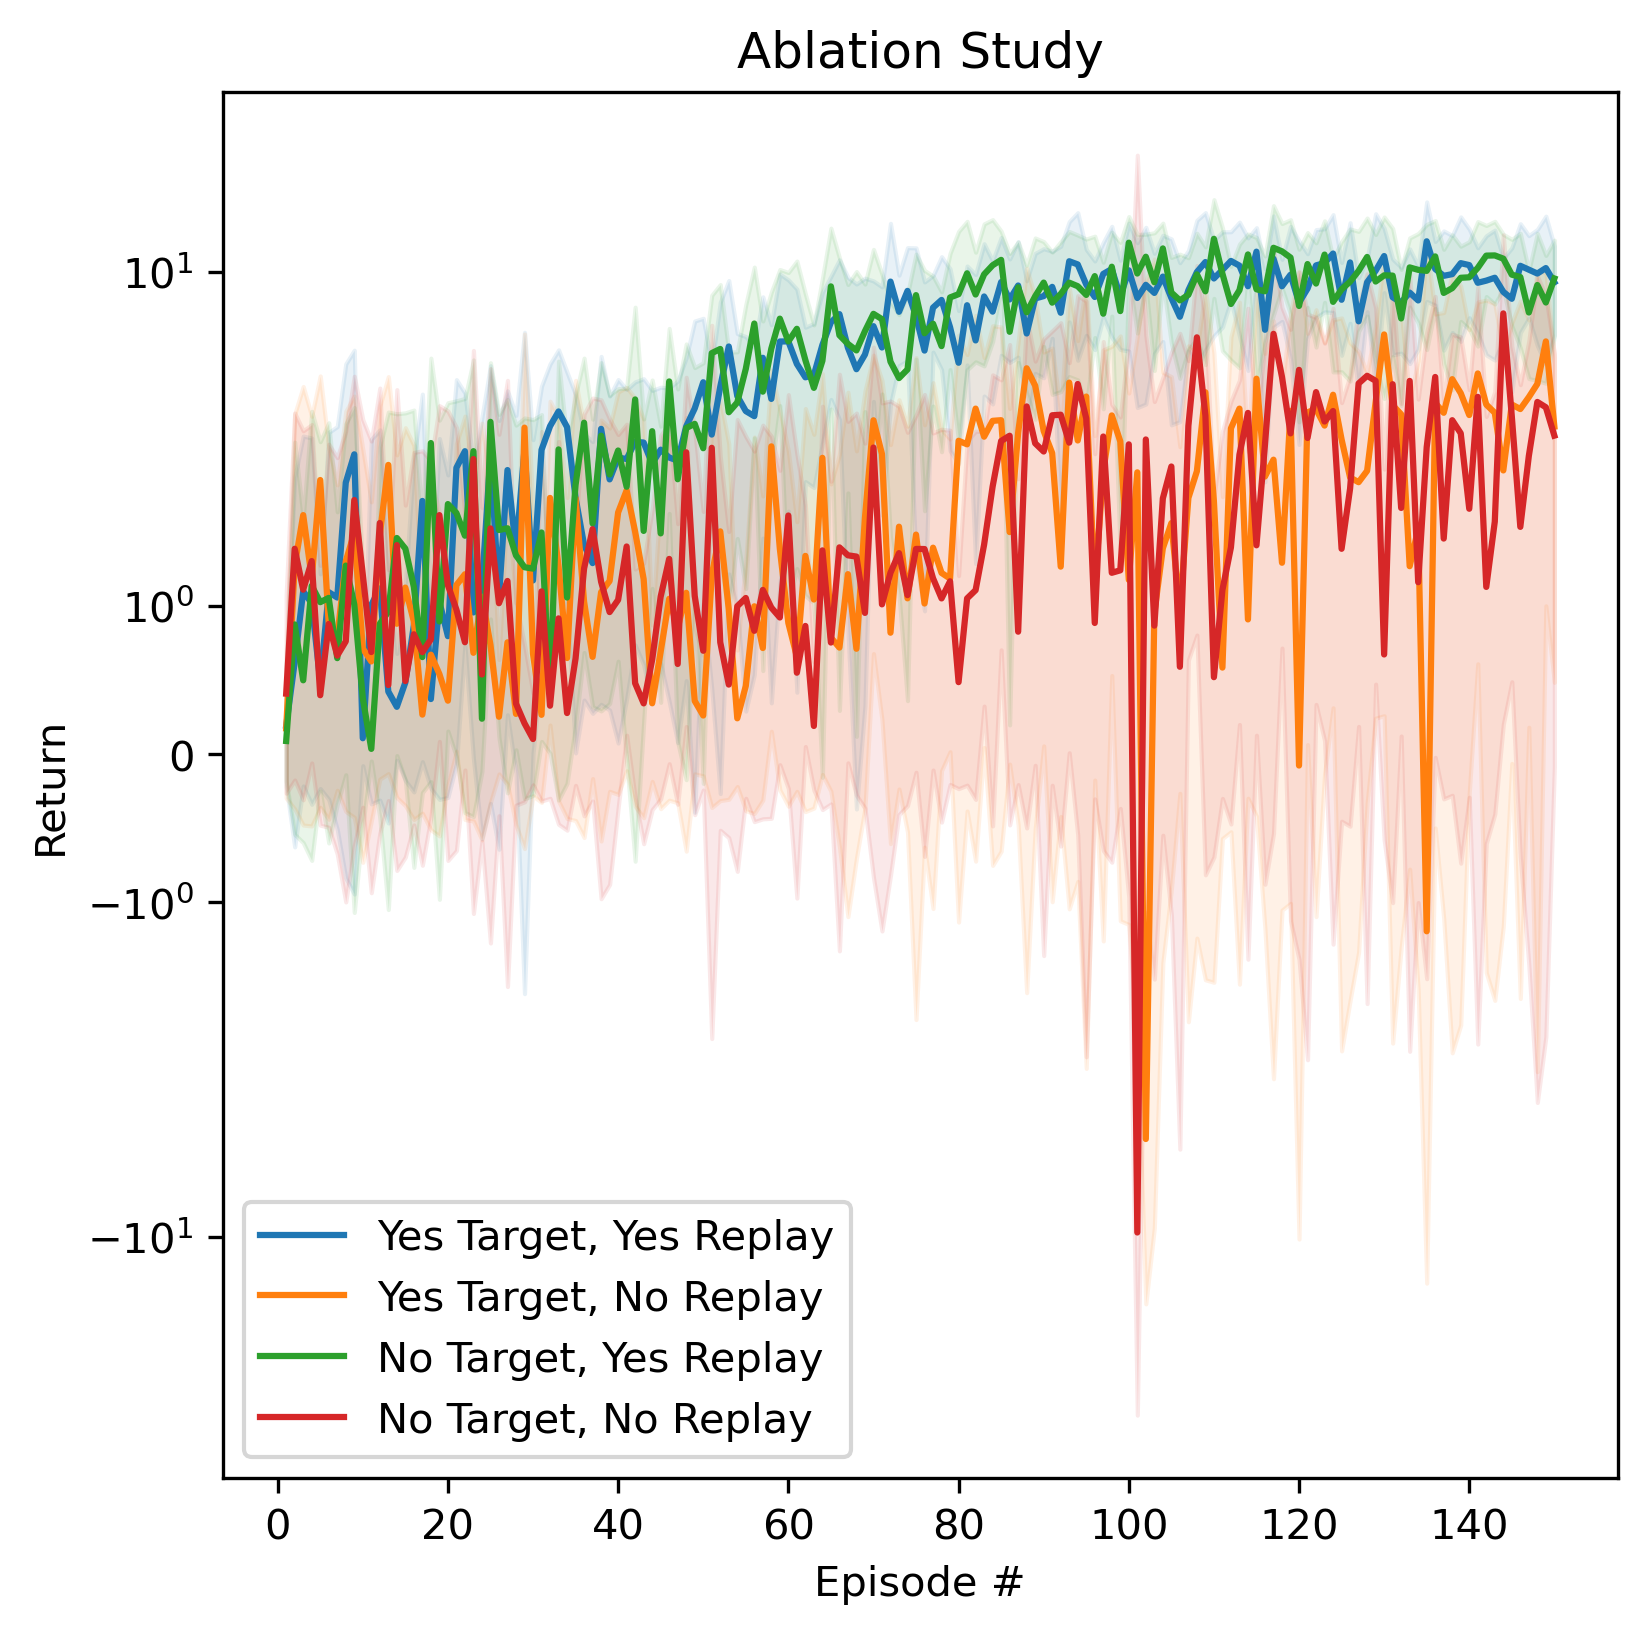
\includegraphics[width=\linewidth]{../figures/results/mean_return_ablation_study_log_True.png}
\caption{Mean return and 1-sigma bounds for 10 runs of the four DQN algorithms on a log scale}
\label{fig:ablation_study_log}
\end{figure}
\begin{figure}[h]
\centering
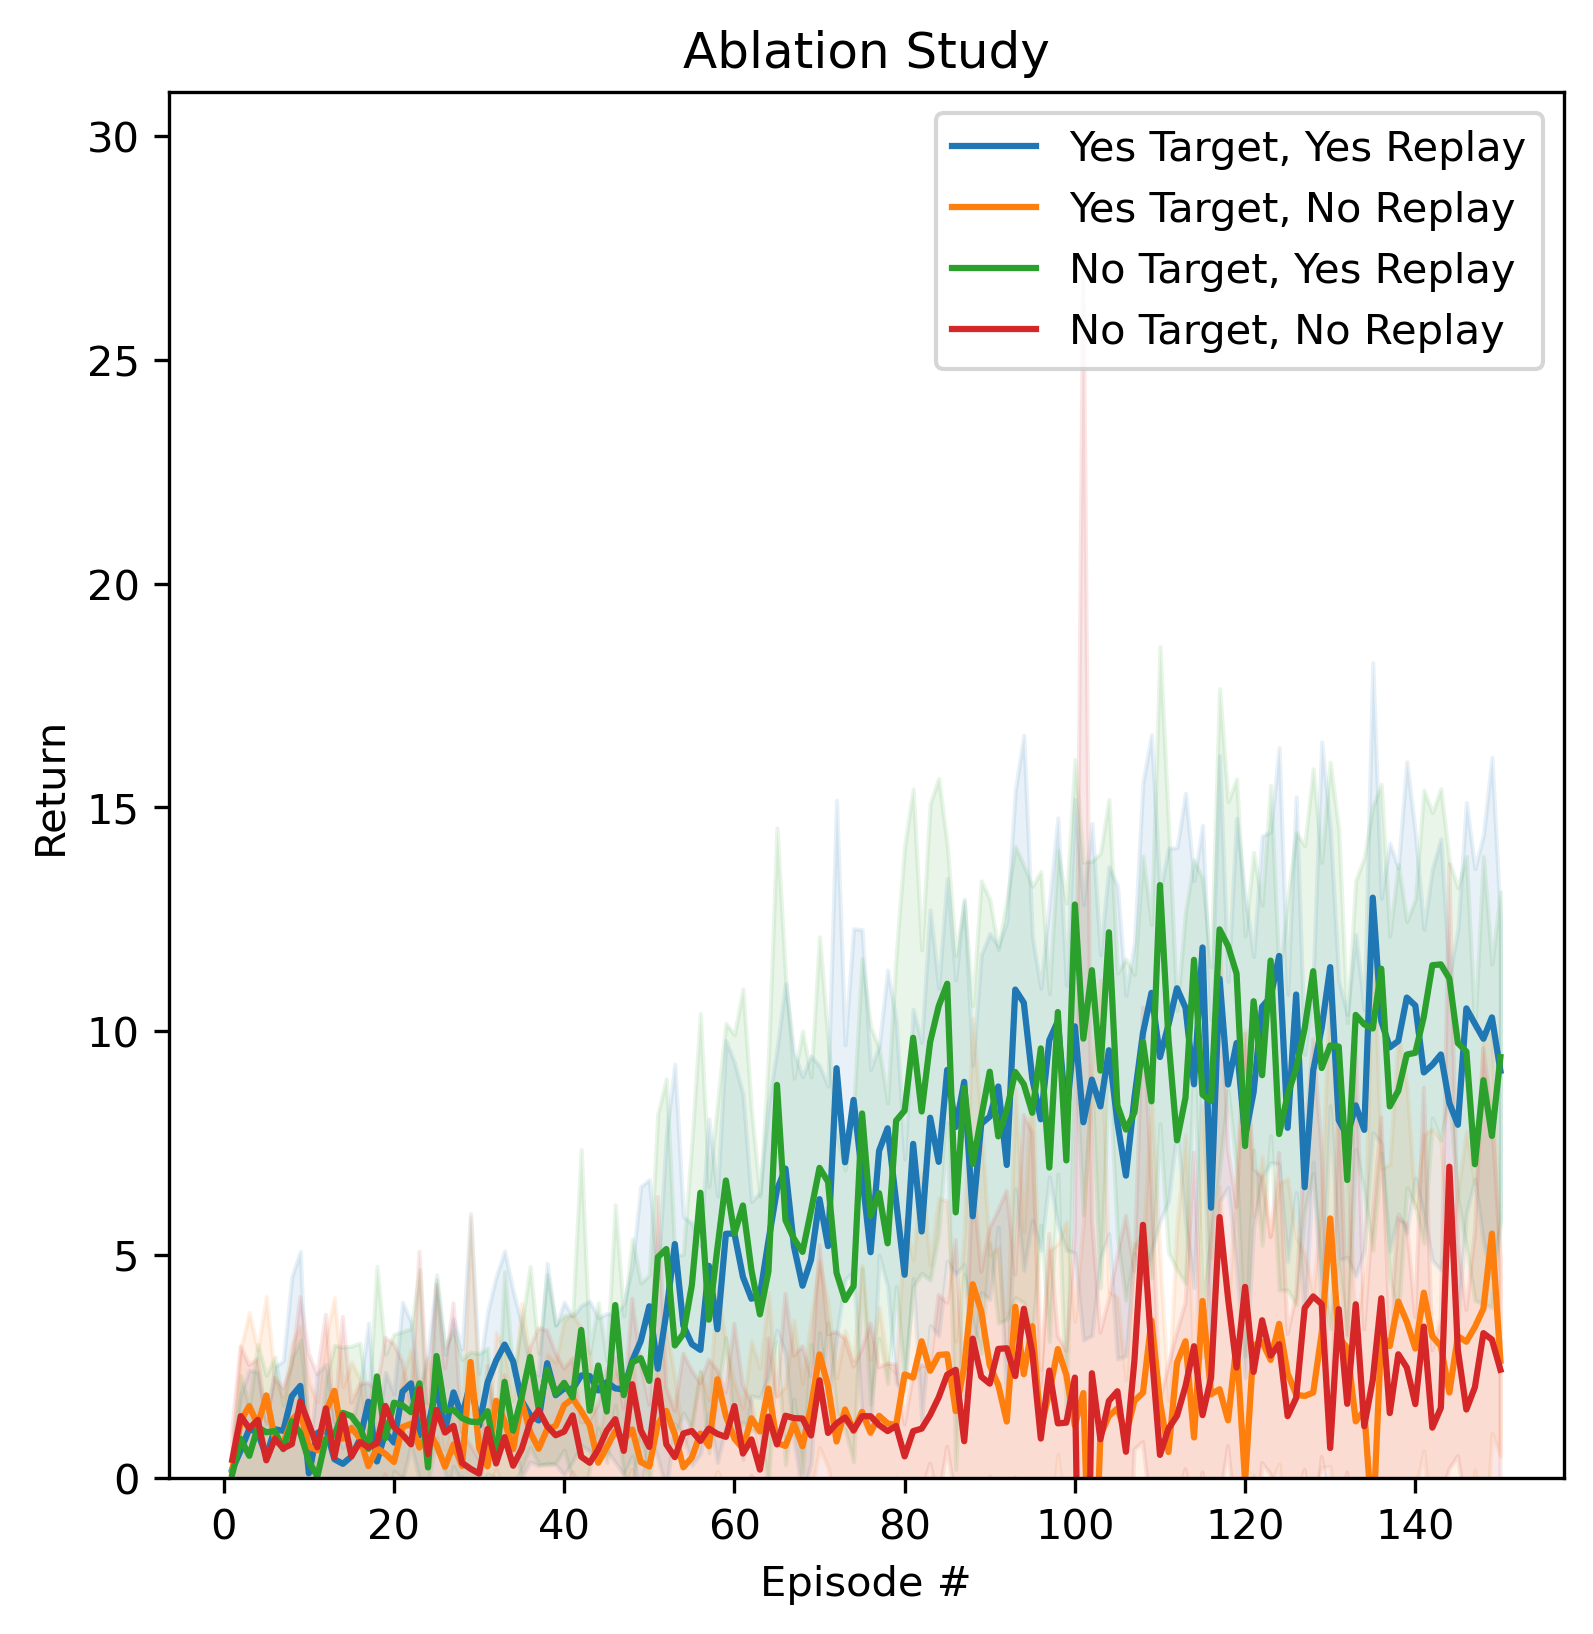
\includegraphics[width=\linewidth]{../figures/results/mean_return_ablation_study_log_False.png}
\caption{Mean return and 1-sigma bounds for 10 runs of the four DQN algorithms on a linear scale (cutoff at 0)}
\label{fig:ablation_study_linear}
\end{figure}
The ablation study clearly suggests that the standard DQN algorithm and the DQN algorithm without a target network perfor significantly better than the DQN algorithm without experience replay and the DQN algorithm without experience replay or target network.

\section{Conclusions}
The inverted pendulum problem was solved using four implementations of the standard DQN algorithm \cite{b1}. Results from these algorithms show that updating the target network at every step is not necessary. However, the experience replay is a significant factor in ensuring that the network learns the policy and remembers it. This remembering is why the two models with experience replay do not have massive negative rewards after initially achieveing some successful outcomes.

\begin{thebibliography}{00}
\bibitem{b1} V. Mnih, K. Kavukcuoglu, D. Silver, A.A. Rusu, J. Veness, M.G. Bellemare et al., ``Human-level control through deep reinforcement learning,'' Nature, vol. 518, pp. 529--533, February 2015.
\end{thebibliography}

\end{document}
